%\titlespacing*{\chapter}{0pt}{\baselineskip}{*3}
\chapter{Analysis}
\label{chap4}

We simultaneously model the resolved 850$\,\mu m$ visibilities from ALMA with the unresolved Spectral Energy Distribution (SED) in order to constrain basic geometric properties of the disk and determine the characteristics of the constituent dust grains. The SED, which describes the flux of the system as a function of wavelength, is dominated by emission from the stellar photosphere at $\lambda$ $\lesssim 5\,\mu m$ (for a debris disk), but the dust in the disk contributes the majority of the flux at $\lambda$ $> 5\,\mu m$. The temperature of the grains can be estimated from the wavelength at which the flux peaks, but because grain size and grain location are degenerate from a modeling point of view, characterizing the grain size distribution is impossible without spatially resolved information. Our ALMA data, able to resolve the dust morphology, provide the means with which to break this degeneracy. 

The main factor that determines the appearance of a model disk image is $\Sigma$(r), the surface density as a function of radius. The simplest description of the surface density is with a single power law such that $\Sigma$(r) $\propto r^{-p}$ with abrupt cutoffs at the inner radius ($R_{In}$) and outer radius ($R_{Out}$). This model is presented in Section \ref{SinglePowerSED_Model}. However, 49 Ceti seems to show a ring-like structure at r $\sim$ 100\,AU, suggesting a more complex model of the surface density could provide a better fit. A simple power law with a narrow density enhancement to mimic this ``ring" is discussed in Section \ref{USDE}, and a double power law, with surface density increasing to the radius of this ``ring" before decreasing, is presented in Section \ref{DP}. 

We use the $\chi^{2}$ parameter to determine the goodness of fit for each model and an affine-invariant Markov Chain Monte Carlo (MCMC) fitting process (\cite{Fore13}, \cite{Good10}, described in Section \ref{MCMC}), to obtain a robust, statistical characterization of the model parameters. The complex interferometric points that ALMA measures, called visibilities, are the result of short ($\sim$ 30\,s) integrations. Each independent baseline, of which there are $N(N-1)/2$ of in an array with N antennas (378 from our 28 element array), produces multiple data points for each integration. Multiple spectral windows, each with adjustable channel resolutions, can be find tuned depending on the requirements of the observation. As discussed in Section \ref{ALMA Observations}, three spectral windows, two with 128 channels and one with 3840 channels, were averaged into single data points to make modeling simpler and more efficient. Taking into account the two orthogonal polarizations detected by the ALMA antennas and after removing flagged visibilities (bad data points) we were left with 131400 visibilities. For these data, the $\chi^{2}$ is calculated as:

\begin{equation}
\chi^{2}_{Vis} =  \sum_{i=1}^{131400} w_{i} \bigg[\bigg(d_{i,real} - m_{i,real}\bigg)^{2} + \bigg(d_{i,imag} - m_{i,imag}\bigg)^{2}\bigg] 
\end{equation} 

where $w_{i}$ is the weight from the data associated with visibility $i$, $m_{i,real}$ and $m_{i,imag}$ are the real and imaginary components of the model visibility $i$, and $d_{i,real}$ and $d_{i,imag}$ are the real and imaginary components of the data visibility $i$. The weight $w_{i}$ given to each visibility is related to the antenna temperature of each antenna in a given baseline, the integration time, and the bandwidth of observation. However, the National Radio Astronomy Observatory (NRAO), which oversees ALMA, was having issues with its proprietary software package CASA (Common Astronomy Software Applications) at the time we were reducing the data, resulting in the weights being scrambled when the data were exported. As a result, we had to recalculate the weights directly from the scatter between channels for visibilities in each un-averaged spectral window. This is possible because the standard deviation from the mean over all channels for each visibility, $\sigma_{i}$, determines $w_{i}$, as $w_{i} = \sfrac{1}{\sigma_{i}^{2}}$. In other words, high quality data points, with only a small amount of scatter between the channels, will have a greater effect in describing the goodness of fit of a given model. 

For the SED, we only fit to data points at wavelengths greater than 5$\,\mu m$, as this is the regime in which the disk contributes a significant flux to the total. A total of 19 points were fit to in the SED until additional photometry from \cite{Robe13} were discovered, at which point 30 points were fit to. Then, the disk $\chi^{2}$ is calculated as:

\begin{equation}
\chi^{2}_{SED} =  \sum_{i=1}^{19~\text{or}~30} \big(\frac{F_{\lambda_{i},model} - F_{\lambda_{i},data}}{\sigma_{\lambda_{i}}}\big)^{2}
\end{equation} 

where $F_{\lambda_{i},model}$ is the model flux, $F_{\lambda{i},data}$ is the data flux, and $\sigma_{i}$ is the error for a measurement at $\lambda_{i}$. The uncertainties associated with the SED data points are small compared with those associated with each visibility, but the large number of visibilities relative to the number of SED fluxes means that each contributes roughly equally to the final result of a simultaneous fit for a suitable model. 

%each ends up contributing almost equally to the final result in a simultaneous fit. 


%With these data constraining the location of the emitting grains and the SED determining the temperature of the grains in a simultaneous model, 
%, but at longer wavelengths, emission from grains in the disk dominate, as the dust grains absorb energetic stellar radiation, heat up, and re-emits a portion of the energy at a wavelength that is dependent on 

\section{Markov Chain Monte Carlo Simulations}
\label{MCMC}

In order to analyze how successful our models are and explore the uncertainties associated with each parameter, we utilize the affine-invariant Markov chain Monte Carlo (MCMC) fitting technique as described by \cite{Good10} and implemented in Python as \texttt{emcee} by \cite{Fore13}. Using a MCMC method allows us to probabilistically sample the full parameter space described by our models, obtain a best-fit result, and get statistically robust error bars by characterizing the full posterior distribution function for each parameter. 

This process works by unleashing a series of model ``walkers," with values for parameters in each model sampled as Gaussians around a user-specified center position (a best guess, generally) and user-specified width. $\chi^{2}$ values are calculated for each model, and the walkers move around parameter space, with the probability of the move being accepted related to the total $\chi^{2}$ of that model. If the $\chi^{2}$ is lower for the next step, the move is accepted. If the $\chi^{2}$ is higher, the probability of that move being made is $e^{-(\sfrac{\Delta \chi^{2}}{2})}$, with $\Delta \chi^{2}$ = $\chi^{2}_{original}$ - $\chi^{2}_{proposed~model}$. Defined as such, models move toward a best-fit from their original locations in parameter space while filling out a full posterior distribution function for each parameter. The position of each walker in parameter space along with its corresponding $\chi^{2}$ for all steps is called a ``chain," and is saved for further use. \texttt{emcee} is affine-invariant, meaning moves are only proposed along lines between the walkers. This makes it more efficient at sampling degeneracies between parameters. 

\begin{figure}
\centering
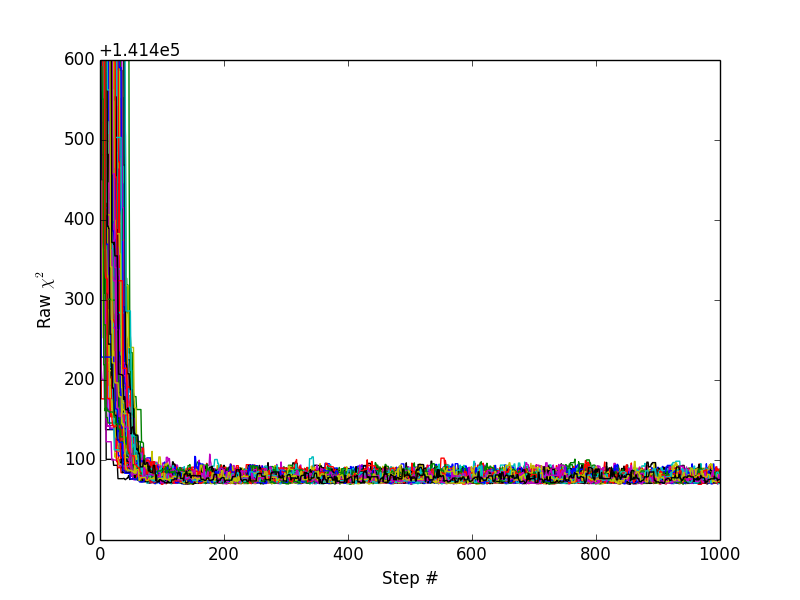
\includegraphics[width = 1\textwidth]{49CET_BurnIn_140x1000_Simplest.png}
\caption{The burn-in and subsequent leveling off of the chi-squared after $\sim$ 100 steps is seen in this plot. Raw $\chi^{2}$ are saved for each step in the chain, and are plotted for each walker (different colors). This burn-in diagram corresponds to the model presented in Section \ref{SinglePowerSED_Model}, which unleashed 140 walkers for 1000 steps.}
\label{fig:49CET_BurnIn}
\end{figure}

\begin{figure}
\centering
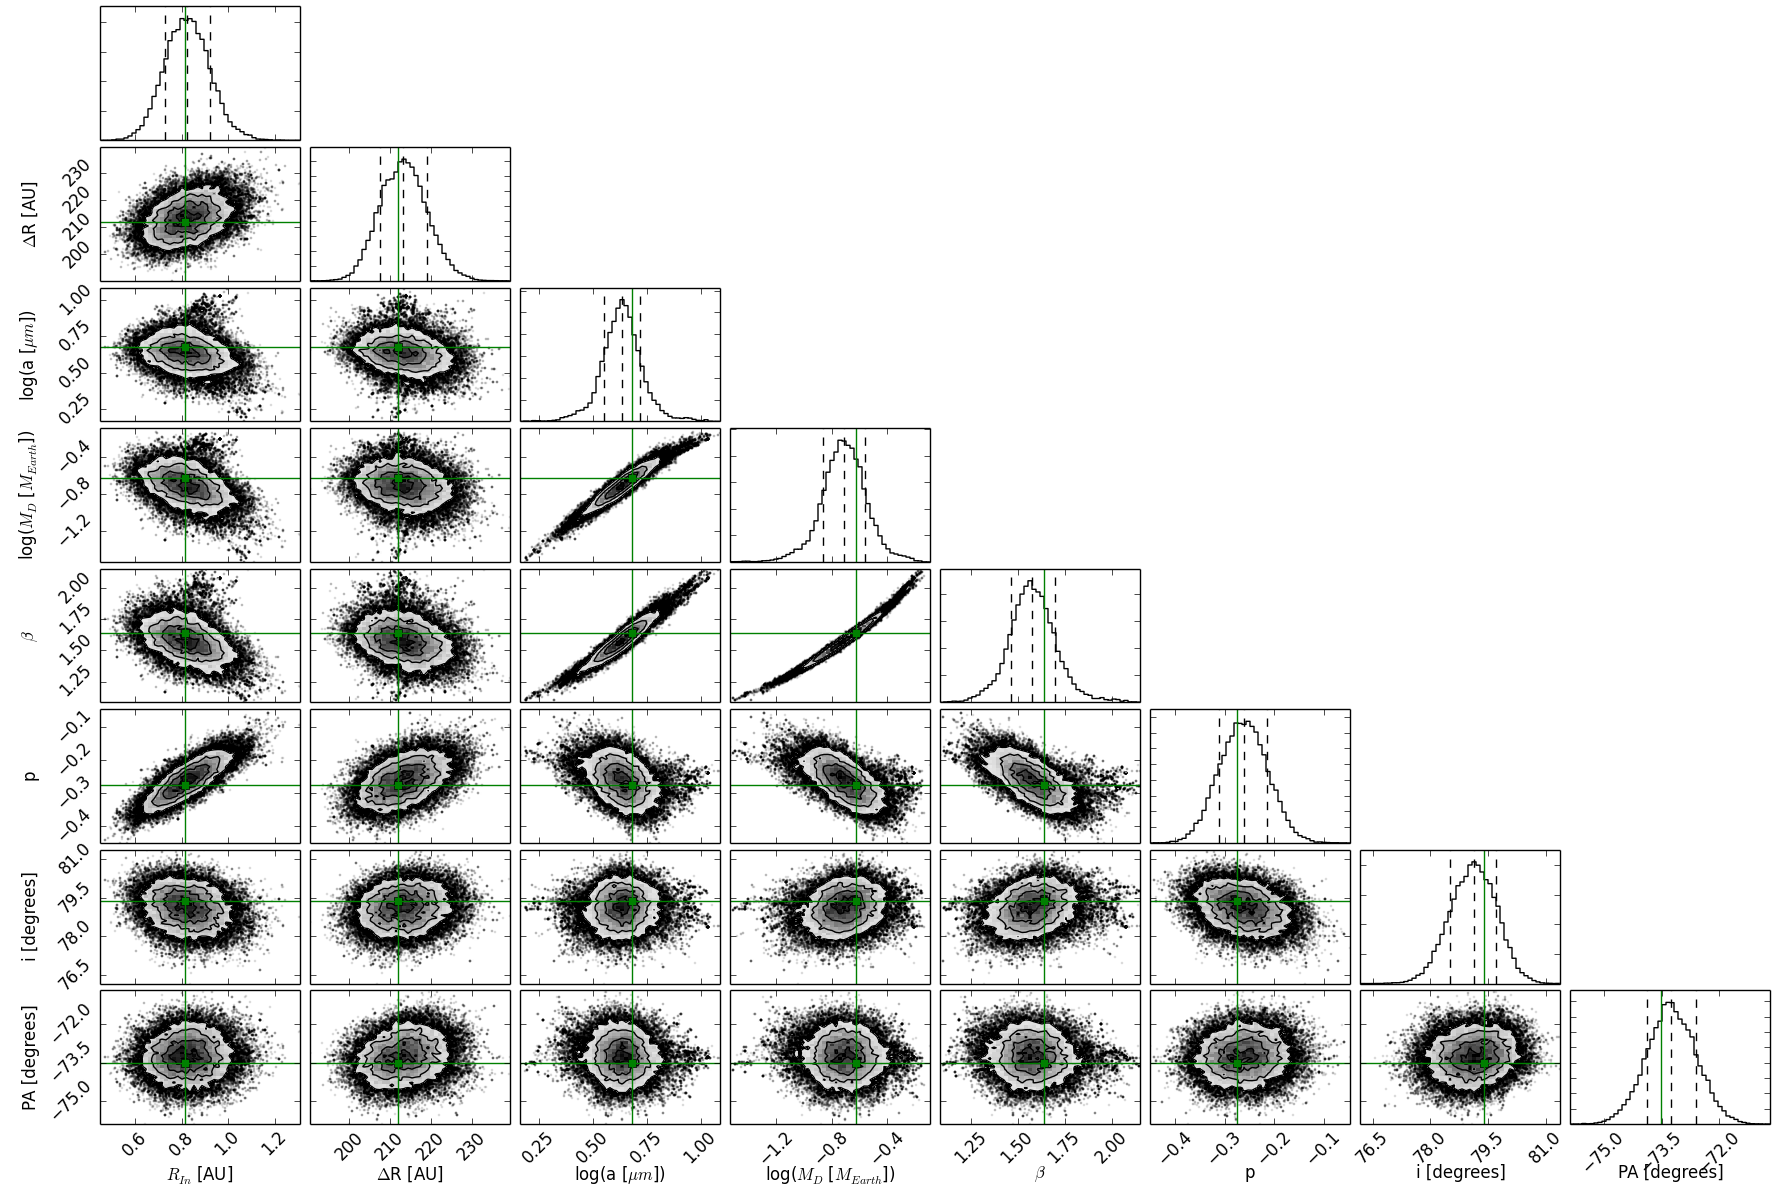
\includegraphics[width = 1\textwidth]{49CET_140x1000_Triangle_150StepBurnIn.png}
\caption{Both one and two dimensional posterior probability distributions for parameters of the single power law model (Section \ref{SinglePowerSED_Model}) as derived from the MCMC chain. The histograms, along the diagonal, display the marginalized distributions for each parameter independently. The dashed lines in the histogram display -1$\sigma$, the median value, and +1$\sigma$ of the distribution, while the green line displays the value of that parameter associated with the overall minimum $\chi^{2}$. The distributions are mostly symmetric. The other plots display the two dimensional marginalized distributions for each pair of parameters and demonstrate the covariances between each pair.}
\label{fig:49CET_Triangle}
\end{figure}

The first $\sim$ 100 steps of an MCMC run compromise the ``burn-in" phase, during which the raw $\chi^{2}$ quickly falls as the walkers move toward the best fit (see Fig \ref{fig:49CET_BurnIn}). This phase tends to be longer if the initial value for one or more of the parameters is far from the correct best-fit value. Before using MCMC, a ``chi-by-eye" fit was performed, with parameters guessed and adjusted until a reasonable fit to the data is found. Then, initial MCMC runs were seeded with wide Gaussians such that the best-fit is somewhere nearby and the MCMC process doesn't have a hard time finding it. Once a best-fit is known, narrower Gaussians are utilized to lessen the burn-in phase.

The median reported value in each table is the most likely value in the MCMC chain once the burn-in phase has been removed; the best-fit value for each parameter corresponds to the global minimum of the total $\chi^{2}$. As the models trace out posterior distribution functions, values $\pm$ 1$\sigma$ from the median value are also reported. We find that the best-fit values are generally within $\pm$ 1$\sigma$ of the median. Figure \ref{fig:49CET_Triangle} shows one and two dimensional posterior distributions from the model presented in Section \ref{SinglePowerSED_Model}.

For all models, disk mass parameters ($M_{Disk}$, $M_{Inner Disk}$, $M_{Outer Disk}$, $M_{Ring}$) and the grain size $a$ are sampled logarithmically, while the rest of the parameters are sampled in a linear fashion.  Visibility-only fits were performed for each model of the surface density such that $\chi^{2}$ = $\chi^{2}_{Vis}$ in order to determine what the spatially resolved data tell us, uninfluenced by the SED. Then, simultaneous fits were performed, with $\chi^{2}$ = $\chi^{2}_{Vis}$ + $\chi^{2}_{SED}$ such that all model parameters could be constrained.

%In Section \ref{SinglePowerSED_Model} we attempted to recreate the data with a standard power law model of the surface density distribution of a geometrically and optically thin dust disk, and while this provided a good fit to the SED, it failed to recreate the visibilities. From the significant positive residuals apparent to the SW side of the disk and negative residuals visible near the center, it was clear that a more complex model describing the surface density was necessary. In Section \ref{MoreComplexModels}, we modeled the surface density both with a double power law, increasing in density to a variable radius before dropping off, and with an unresolved surface density enhancement at a variable radius. Both models were able to recreate the SED, but the SED dominated the fit, skewing the fits to the visibilities. In order to create the significant mass of hot dust necessary to recreate the mid-IR excess, the best-fit results had inner radii within 1AU of the star, resulting in models that were too bright at the center. The unresolved surface density enhancement (USDE???) model was able to account for the ring-like structure, but the double power law model was not, presumably altered by the fit to the SED. 

%To eliminate the contribution of the SED, $\chi^{2}$ values were computed only using the visibilities for both the double-power law and the surface density enhancement. As presented in Section \ref{VisOnly}, we found that both models were able to recreate the density enhancement without becoming too bright at the center. However, as expected, these models didn't contribute enough flux at mid-IR wavelengths. Building upon the results of \cite{Wahh07}, we described an inner disk with a grain size of 0.1$\,\mu m$ and let the characteristic grain size of the outer belt vary. Because small grains radiate at higher temperatures at a given distance from the star than their larger brethren, they were able to boost the mid-IR flux without contributing significantly to the flux at millimeter wavelengths. Both the double power law and unresolved surface density enhancement models with different characteristic grain sizes, presented in Section \ref{ThreePart}, were able to fully recreate our data. 

%Best fit parameters were determined using an affine-invariant Markov Chain Monte Carlo (MCMC) fitting algorithm (\ref{Fore13}, Goodman \& Weare 2010 <<no bibtex for this??, described in Section \ref{MCMC}), a process that provides a robust, statistical characterization of the model parameters. 

%A closer look at the mid-IR spectrum of 49 Ceti gathered from IRS is presented in Section \ref{MidIR}. 

%%%%%%%

\section{Single Power Law Model}
\label{SinglePowerSED_Model}

In order to model a simple geometrically and optically-thin disk model, we follow the approach of \cite{Rica13}, and have the surface density profile $\Sigma(r)$ described by a single power law $p$, with abrupt cutoffs at the inner radius, $R_{In}$, and the outer radius, $R_{Out}$. The surface density is normalized to 100\,AU ($\Sigma_{100\text{AU}}$) and parameterized as:

\begin{equation}\label{eq:sigmaR}
\Sigma(r) = \Sigma_{100\text{AU}}\Big(\frac{r}{100\text{AU}}\Big)^{-p}
\end{equation}

We are able to solve for $\Sigma_{100\text{AU}}$, as we know the integral of the surface density over all infinitesimal rings from $R_{In}$ to $R_{Out}$ must be equal to the total mass of emitting grains in the disk, $M_{Disk}$. 

\begin{equation}\label{eq:mdisk}
M_{Disk} = \int_{R_{In}}^{R_{Out}} \Sigma(r) 2 \pi r \,dr = \int_{R_{In}}^{R_{Out}} \Sigma_{100\text{AU}}\Big(\frac{r}{100\text{AU}}\Big)^{-p} 2 \pi r \,dr
\end{equation}

Integrating and solving for $\Sigma_{100\text{AU}}$, we find:

\begin{equation}\label{eq:sigma100}
\Sigma_{100\text{AU}} = \cfrac{M_{Disk} (2 - p)}{2\pi (100\text{AU})^{p} [(R_{Out})^{2-p}-(R_{In})^{2-p}]}
\end{equation}

Equation \ref{eq:sigma100} lets us vary $p$, $R_{In}$, $R_{Out}$, and $M_{Disk}$. We model $R_{Out}$ as $R_{In} + \Delta R$ to easily ensure that $R_{Out}$ doesn't go within $R_{In}$. Combining these parameters with Equation \ref{eq:sigmaR}, we are able to calculate what the surface density should be at any radius. 

The parameters that describe the dust grains are the characteristic grain size ($a$) and the long-wavelength power law index of grain emission efficiency ($\beta$). We assume that the number of grains of each size is follows the distribution determined in a theoretical collisional equilibrium, i.e. dN $\propto a^{-3.5}$\,d$a$ \citep{Thib07}. The absorption and emission efficiency of a grain as a function of wavelength, $Q_{\lambda}$, is related to size of the grain. Grains are good absorbers and emitters at wavelengths shorter and comparable to their size, but their efficiency drops off as $\lambda^{-\beta}$ at wavelengths larger than their size. We describe $Q_{\lambda} = 1 - e^{-(\frac{\lambda}{2\pi a})^{-\beta}}$, which has $Q_{\lambda} \approx (\sfrac{\lambda}{2\pi a})^{-\beta}$ in the limit of $\lambda$ $>>$ $2\pi a$ and $Q_{\lambda} \approx 1$ when $\lambda$ $<<$ $2\pi a$, which are exactly the properties we desire. 
%%%%%%%%%%%%%%%%%%%%%%%%%%%%%%%%%%%%%%%%%
%%%%%%%%%%%%%%%%%%%%%%%%%%%%%%%%%%%%%%%%%
%%%%%%%%%%%%%%%%%%%%%%%%%%%%%%%%%%%%%%%%%
%%%%%%%%%%%%%%%%%%%%%%%%%%%%%%%%%%%%%%%%%
%%%%%%%%%%%%%%%%%%%%%%%%%%%%%%%%%%%%%%%%%
%%%%%%%%%%%%%%%%%%%%%%%%%%%%%%%%%%%%%%%%%

This parameterization for $Q_{\lambda}$ also mimics a distribution of grain sizes, whereas MCMC analysis would be impossible if we modeled a full distribution of grain sizes due to significant computational inefficiencies. Large values of $\beta$ signify an emphasis on grain sizes $\sim$ $a$, where as smaller values of $\beta$ give more weight to large grains and their emission at longer wavelengths. By smoothly describing the quantum emission efficiency in this way, we end up with a model that is very computationally efficient and is able to recreate the SED with the minimum number of variable parameters. 


%As mentioned earlier, at long wavelengths, the opacity ($\kappa$) of the grains is described by $\kappa \sim \lambda^{-\beta}$ at wavelengths larger than their size\citep{Natt07}.



%This parameterization for $Q_{\lambda}$ has the added advantage that it mimics a distribution of grain sizes, whereas MCMC analysis would be impossible if we modeled a full distribution of grain sizes due to significant computational inefficiencies. Large values of $\beta$ signify an emphasis on grain sizes $\sim$ $a$, where as smaller values of $\beta$ give more weight to large grains and their emission at longer wavelengths. By smoothly describing the quantum emission efficiency in this way, we end up with a model that is very computationally efficient and is able to recreate the SED with the minimum number of variable parameters. 
%%%%%%%%%%%%%%%%%%%%%%%%%%%%%%%%%%%%%%%%%
%%%%%%%%%%%%%%%%%%%%%%%%%%%%%%%%%%%%%%%%%
%%%%%%%%%%%%%%%%%%%%%%%%%%%%%%%%%%%%%%%%%
%%%%%%%%%%%%%%%%%%%%%%%%%%%%%%%%%%%%%%%%%
%%%%%%%%%%%%%%%%%%%%%%%%%%%%%%%%%%%%%%%%%



%Because grains are very inefficient emitters at $\lambda$ $>>$ $2\pi a$, assigning a single grain size for the dust would be insufficient to recreate the contribution of the dust to the SED. 

%\begin{equation}\label{eq:qFn}
%$Q_{\lambda} = 1 - e^{-(\frac{\lambda}{2\pi a})^{-\beta}}$
%\end{equation}

%The combination of these parameters allows us to approximate a grain size distribution; large values of $\beta$ signify a high ratio of small grains to large grains whereas values of $\beta$ close to zero suggest .....which essentially modifies a Rayleigh-Jeans tail to approximate a distribution of grain sizes.  

The temperature of a grain of a given size at a given distance from the star can then be derived by assuming radiative equilibrium between the the stellar radiation absorbed and the energy emitted by the grain. Not taking the albedo of the grains into account, the energy balance is described by:

\begin{equation}\label{EBalance}
\frac{\pi a^{2} L_{\bigstar}}{4 \pi d^{2}} = 4 \pi a^{2} \sigma T_{g}^{4}
\end{equation}

where $a$ is the grain size, $L_{\bigstar}$ is the luminosity of the central star, $d$ is the distance to the grain from the star, $\sigma$ is the Stephan-Boltzmann constant, and $T_{g}$ is the temperature of the grain. Solving for $T_{g}$, we find:

\begin{equation}\label{tEst}
T_{g} \simeq (\frac{L_{\bigstar}}{16 \pi \sigma})^{\sfrac{1}{4}} d^{\sfrac{-1}{2}}
\end{equation}

From this we can see that the temperature of the grains falls off as approximately $d^{\sfrac{-1}{2}}$. However, grains are not perfect absorbers or emitters, and the albedo changes both as a function of wavelength and grain size. To account for this, we model the composition of the dust as compact astrosilicates as described by \cite{Drai03}, and describe the grains' opacity and albedo according to Mie theory (see \citealt{Bohr83}). Taking the absorption and emission efficiency as a function of grain size and wavelength, $Q(a,\lambda)$ into account, the energy balance is described by:

\begin{equation}
\label{eq:fullEBalance}
\frac{1}{4\pi} \int_0^\infty Q(a,\lambda)F_{\lambda}(r,\lambda)\,\mathrm{d}\lambda = \int_0^\infty Q(a,\lambda)B(T,\lambda)\,\mathrm{d}\lambda
\end{equation}

$F_{\lambda}(r,\lambda)$ describes the flux received by a grain at a radius $r$ from the star and wavelength $\lambda$, and $B(T,\lambda)$ is the grains' Planck function. These expressions are numerically integrated to obtain the temperature of a given grain. The left integral is calculated as a function of $a$ at a radius of 50\,AU, and these values are scaled by r$^{\sfrac{-1}{2}}$ to get the value at different radii. The right integral is calculated as a function of both $a$ and $T$. With this setup, we are able to derive an accurate temperature for a grain of size $a$ at a radius $r$ for grains of any size anywhere in the disk. 

%Then, for a grain of size $a$ at a radius $r$, we are able to derive an accurate temperature, thereby allowing the determination  its contribution to the total flux for grains throughout our model of the disk.

We compare our model to the SED of 49 Ceti at observed photometric points gathered from the literature (displayed in Table \ref{tab:SED}) in order to calculate a $\chi^{2}_{SED}$. The SED displays a double-peaked shape (see Figure \ref{fig:49CET_Simple_SED}) that is consistent with emission from a two-belt configuration, with a warm inner belt boosting mid-IR fluxes and a cool outer belt responsible for the second peak at millimeter wavelengths. We model the SED with two components: (1) a Kurucz-Lejeune model photosphere with surface gravity log(g) = 4.5, effective temperature $T_{Eff}$ = 10000K, and solar metallicity Z = 0.01 \citep{Chen06}, and (2) an extended, spatially-resolved debris disk. Points at a wavelength less than 5$\,\mu m$ were not included in the fit, as the disk contributes a negligible flux relative to the star in this regime. 19 points were included in the SED fit for some models before additional photometry was found, at which point all 30 points presented in Table \ref{tab:SED} were used for fitting (all advanced models used for statistical analysis in Section \ref{stats} use all 30 data points). The ALMA flux is not included in the calculation of the SED $\chi^{2}$, as this flux is implicitly included in the creation of the model image at 850$\,\mu m$ that we compare the visibilities to when calculating the visibility $\chi^{2}$. The IRS spectrum originally consisted of 360 points between 5 and 35$\,\mu m$, but was averaged down to 9 for the sake of computational efficiency. The errors reported in the table for these points are the absolute calibration uncertainty (assumed to be 10$\%$ of the flux measurement) and the statistical uncertainty added in quadrature.

\begin{table*}
\caption{Spatially Unresolved Continuum Fluxes Measured for the 49 Ceti System}
%\resizebox{\textwidth}{!}{
\begin{center}
%\begin{multicols*}{2}
%\setlength\columnsep{12pt}
%\def\arraystretch{1}
%\begin{tabular}{1*{5}{c}r}
\begin{tabular}{ccc}
    \hline\hline   
    Wavelength ($\mu m$) & Flux (Jy) & Source & %\multicolumn{1}{p{2cm}}{\centering Number of \\ Antennas} 
    \hline 
    0.38 & 8.68 & Yerkes Observatory, \cite{Cowl69} \\ 
    0.45 & 20.99 & $''$ \\    
    0.55 & 20.52 & $''$ \\     
    1.22 & 9.55 & Michigan Curtis Telescope, \\     
    1.65 & 6.38 & \citet{Houk88} \\     
    2.18 & 3.98 & $''$ \\     
    3.55 & 1.72 & $''$ \\     
    4.77 & 0.96 & $''$ \\
    5.86 & 0.69 $\pm$ 0.07& IRS Spectrum \\ 
    7.07 & 0.48 $\pm$ 0.05&$''$ \\ 
    8.97 & 0.32 $\pm$ 0.03& $''$ \\ 
    11.40 & 0.21 $\pm$ 0.02& $''$ \\ 
    13.90 & 0.18 $\pm$ 0.02& $''$ \\ 
    17.13 & 0.19 $\pm$ 0.02& $''$ \\ 
    20.90 & 0.21 $\pm$ 0.02& $''$ \\ 
    27.21 & 0.35 $\pm$ 0.03& $''$ \\ 
    34.00 & 0.6 $\pm$ 0.1& $''$ \\ 
    11.56 & 0.21 $\pm$ 0.02 & \textit{WISE}, \cite{Wrig10} \\         
    12.0 & 0.33 $\pm$ 0.07 & \textit{IRAS} Faint Source Catalog \\     
    25.0 & 0.38 $\pm$ 0.08 & $''$ \\    
    60.0 & 2.0 $\pm$ 0.4 & $''$ \\     
    100.0 & 1.91 $\pm$ 0.38 & $''$ \\   
    12.5 & 0.20 $\pm$ 0.03 & Keck, \cite{Wahh07} \\   
    17.9 & 0.19 $\pm$ 0.03 & $''$ \\  
    150.0 & 0.8 $\pm$ 0.5 & ISO \\  
    170.0 & 1.1 $\pm$ 0.5 & $''$ \\  
    63.19 & 2.01 $\pm$ 0.35 & Herschel, \cite{Robe13} \\
    70.00 & 2.142 $\pm$ 0.058 & $''$ \\
    72.84 & 1.95 $\pm$ 0.32 & $''$ \\
    78.74 & 1.90 $\pm$ 0.31 & $''$ \\
    90.16 & 1.88 $\pm$ 0.32 & $''$ \\
    145.54 & 1.16 $\pm$ 0.18 & $''$ \\
    157.68 & 0.98 $\pm$ 0.13 & $''$ \\
    160.00 & 1.004 $\pm$ 0.053 & $''$ \\
    250.0 & 0.372 $\pm$ 0.027 & $''$ \\
    350.0 & 0.180 $\pm$ 0.014 & $''$ \\
    500.0 & 0.086 $\pm$ 0.009 & $''$ \\
%    850.0 & ???? $\pm$ ???? & This work \\
    1300.0 & 0.0021 $\pm$ 0.0007 & CARMA, This work \\
        \hline
\end{tabular}
%    \end{multicols*}
    \end{center}
%\end{adjustbox}
\label{tab:SED}
\caption{The 30 fluxes and their corresponding uncertainties gathered from the literature.}
\end{table*}

In addition to describing and fitting the flux contribution of the grains to the SED, we simultaneously create a high-resolution model image of the disk at 850$\,\mu m$, the wavelength of the spatially-resolved ALMA observations. These images have a resolution on the order of 10$\%$ the spatial scale sampled by our longest baseline, i.e. 3\,AU/pixel. However, for the model described in Section \ref{USDE}, which contained a narrow ring, we used model images with a resolution of 1.5\,AU/pixel. These model images are sampled at the same baseline separations and orientations as the ALMA observations using the MIRIAD command \texttt{uvmodel}, allowing us to compare our model disk to the data. We do this in the visibility domain rather than with the data and model images. These images, which have been created from the visibilities using the the non-linear \texttt{clean} algorithm, do not have well characterized uncertainties, whereas the noise is well understood for each visibility in the visibility domain \citep{Schw78_clean}. In addition, fitting to the visibilities preserves information from the longest baselines (corresponding to the smallest angular scales), whereas the resolution of the image is always coarser than the smallest angular scale.
 
% From this process, the noise that is well understood for each visibility in the visibility domain and is hard to  estimate in the image domain \citep{Schw78_clean}, preventing us from characterizing the uncertainties in the image domain.
 

%a non-linear process that doesn't preserve the 
%noise properties of vis weights....
%understand noise in vis but not in image- clean is nonlinear- 
%visibilities preserve info on smallest scales- long baselines - because clean beam is always larger than smallest angular scale in data (somewhat) over all baselines
%weights associated with ......?????????
%Although there are significantly more visibilities (141300) than SED points that we fit to (30), the visibilities have much lower signal-to-noise, meaning the weight that each $\chi^{2}$ has on the final fit is roughly equal. 

\subsection{Visibility-only Fit}
\label{simple_VisOnly}

In order to ascertain what physical parameters can describe the ALMA data, we perform MCMC analysis using only the visibility $\chi^{2}$. As seen in Figure \ref{fig:49CET_Simple_Vis_ModelResidual}, the model is a good fit, with just a small scatter of 2$\sigma$ residuals left in the residual image. We find that large grains ($\sim$ 850$\,\mu m$), which dominate emission at the wavelength of the ALMA image, are not found within $\sim$ 70\,AU, and that the disk extends out to $\sim$ 300\,AU. Without the simultaneous fit to the SED, $M_{Disk}$, $\beta$, and $a$ are not well constrained.

Even though we didn't take the SED $\chi^{2}$ into account in this model, it is an enlightening exercise to examine what the SED looks like with these model parameters. As seen in Figure \ref{fig:49CET_Simple_Vis_SED}, the model seems to fit the secondary peak from the disk emission (just by chance), but is clearly not bright enough in the mid-infrared. A population of hotter dust grains is necessary to recreate this mid-IR deficit. 

\begin{figure}[t!]
\centering
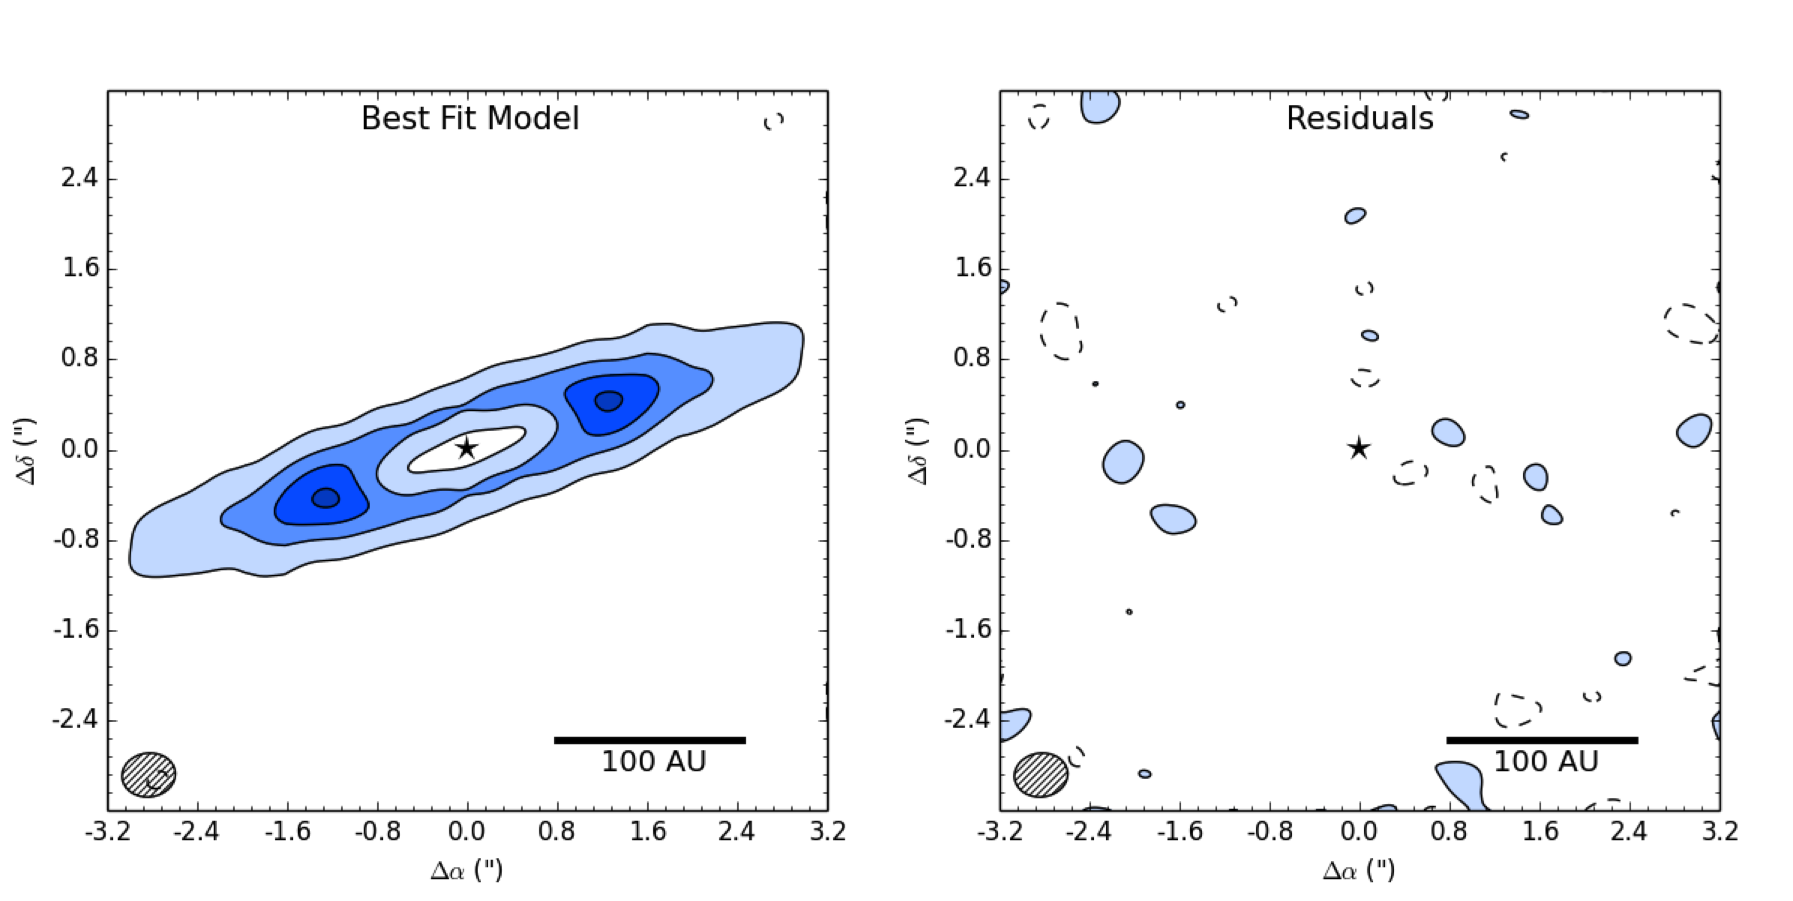
\includegraphics[width = 1\textwidth]{49CET_Simple_Vis_ModelResidual.png}
\caption{The model image (left) and residuals (right) for the single power law model fitting just the visibilities. The residuals are the ALMA visibilities minus model visibilities, subtracted in the visibility domain, then imaged. Contours are [-2, 2, 4, 6, 8] $\times$ 58$\,\mu$Jy (the RMS noise of the data image).}
\label{fig:49CET_Simple_Vis_ModelResidual}
\end{figure}

\begin{figure}
\centering
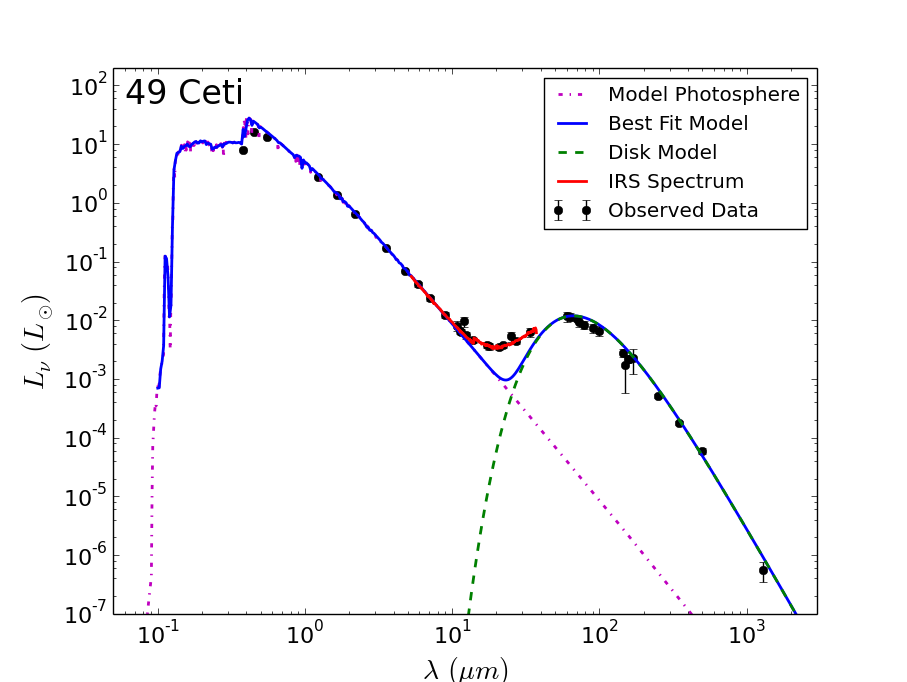
\includegraphics[width = 1\textwidth]{49CET_Simple_Vis_SED_AllData.png}
\caption{The model SED created from parameters derived from the visibility-only single power law fit.}
\label{fig:49CET_Simple_Vis_SED}
\end{figure}

\begin{table}
\begin{center}
    \def\arraystretch{1.37}%
    \begin{tabular}{l*{2}{c}r}
    \hline
    Parameter & Median Value $\pm$ 1$\sigma$ & Best Fit Value \\ \hline
     $R_{In}$  [AU] & 70$^{+3}_{-3}$ & 69\\  
     $\Delta R$ [AU] & 245$^{+9}_{-9}$ & 243\\ 
     log($M_{Disk}$ [$M_{\oplus}$]) & -0.8$^{+0.8}_{-0.8}$ & -0.7 \\
     log(a [$\mu$m]) & 0.8$^{+0.5}_{-0.5}$ & 0.4\\ 
     $\beta$ & 1.4$^{+0.6}_{-0.6}$ & 1.4\\ 
     $p$ & 1.21$^{+0.13}_{-0.17}$ & 1.24\\ 
     $i$ [$^\circ$] & 79.6$^{+0.4}_{-0.4}$ & 79.5 \\ 
     $PA$ [$^\circ$] & -71.3$^{+0.5}_{-0.5}$ & -71.3\\
    \hline
    \end{tabular}
\end{center}
\caption{The median and best fit values for the single power law model fitting only the visibilities.}
\label{tab:49CET_Simple_Vis_Table}
%for all parameters of the model of 49 Ceti's dust disk. THIS IS SIMPLE BONUS BELT, JUST VIS100x840}
\end{table}


\subsection{Simultaneous SED and Visibility Fit}
\label{Simple_SED_Vis}

\begin{figure}[t!]
\centering
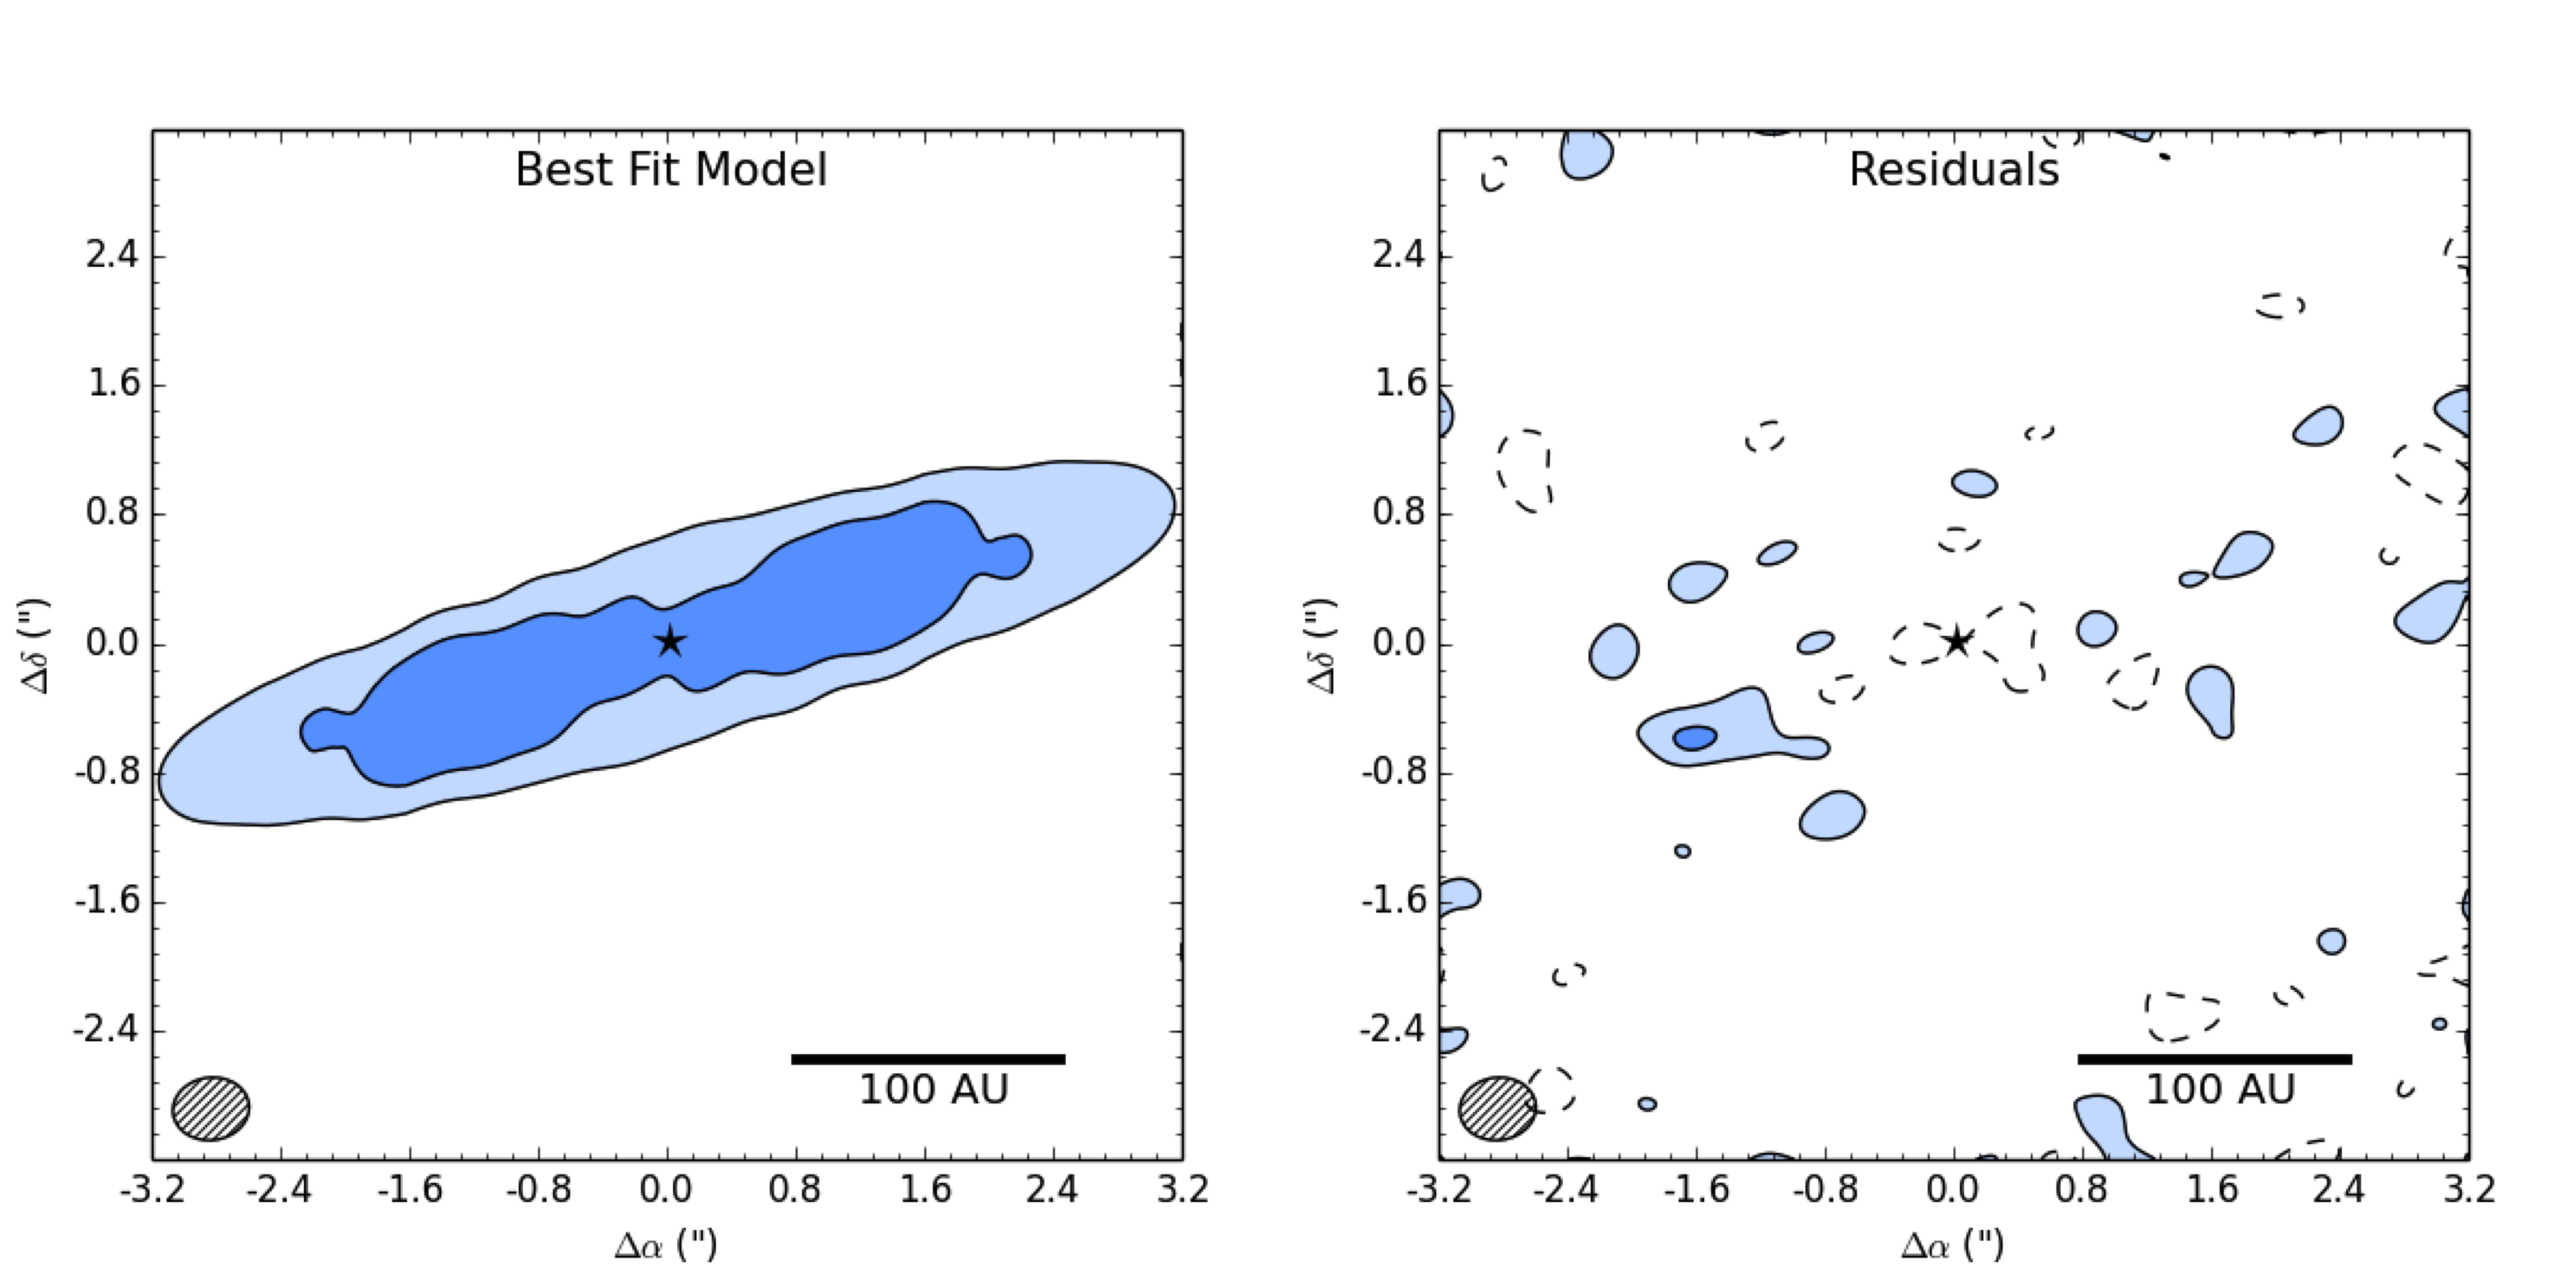
\includegraphics[width = 1\textwidth]{49CET_Simple_ModelResidual.png}
\caption{The model image (left) and residuals (right) for the single power law model fitting to both the SED and visibilities. Contours are [-2, 2, 4] $\times$ 58$\,\mu$Jy (the RMS noise of the data image). The model fails to account for the region of higher density on the southeast side of the disk and leaves residuals in a ring-like pattern around the disk. It is also slightly too bright at the center.}
\label{fig:49CET_Simple_ModelResidual}
\end{figure}

Using the same single power law description of the surface density, we perform a simultaneous fit to both the visibilities and the SED. The best-fit model and residual images are presented in Figure \ref{fig:49CET_Simple_ModelResidual}, the best-fit SED is plotted in Figure \ref{fig:49CET_Simple_SED}, and the parameters are displayed in Table \ref{tab:SimpleModel_Table}. The inner radius in this model is $\sim$ 1\,AU, which has created enough hot grains to recreate the mid-IR fluxes, and the rest of the SED is also a very good fit. However, in doing so, the model has deviated considerably from the value of $p$ that worked well for the visibility-only best-fit model, with $p$ = $-$0.27 now instead of $p$ = 1.24. This difference is clearly due to the influence of the SED and the need for a non-zero inner disk surface density to create hot grains to recreate the mid-IR excess. The shallowly increasing value of $p$ suggests the model is trying to juggle the need of $\Sigma_{Outer Disk} > \Sigma_{Inner Disk}$, and as can be seen in Figure \ref{fig:49CET_Simple_ModelResidual}, this balance is imperfect and results a model disk that is too bright in the center and not bright enough farther out.

%The model leaves 2$\sigma$ residuals in a ring, suggesting the need for a description of the surface density that peaks at a variable radius. It is also too bright near the center of the disk. The median and best-fit values for the single power law  model are presented in Table \ref{tab:SimpleModel_Table}.

\begin{figure}%[!]
\centering
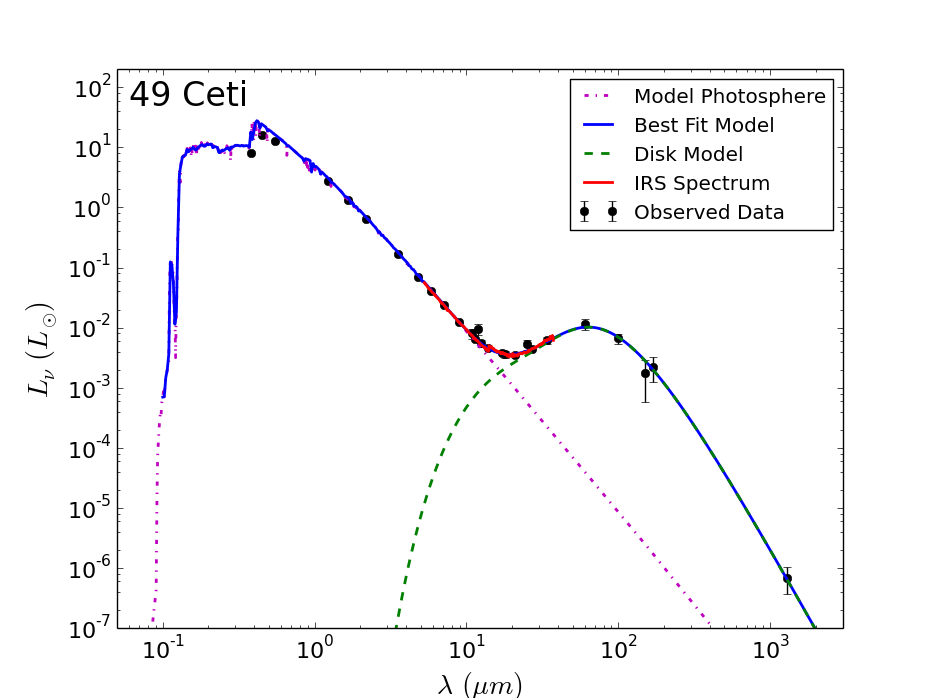
\includegraphics[width = 1\textwidth]{49CET_Simple_SED.png}
\caption{The best fit SED of 49 Ceti for the single power law model simultaneously fitting the SED and visibilities. The best fit model is the sum of the disk model and the model photosphere. Photometric points, excluding those from \cite{Robe13}, are taken from the literature. The full IRS spectrum is presented for display purposes.}
\label{fig:49CET_Simple_SED}
\end{figure}

\begin{table}%[t!]
\begin{center}
    \def\arraystretch{1.10}%
    \begin{tabular}{l*{2}{c}r}
    \hline
     Parameter & Median Value $\pm$ 1$\sigma$ & Best Fit Value \\ \hline
     $R_{In}$  [AU] & 0.82$\pm$0.10 & 0.81\\ 
     $\Delta$R [AU] & 213$\pm$6} & 212 \\ 
     log(a [$\mu$m])  & 0.63$\pm$0.10 & 0.68\\ 
     log($M_{Disk}$ [$M_{\oplus}$])  & -0.71$\pm$0.15 & -0.63\\ 
     $\beta$ & 1.58$\pm$0.12 & 1.64\\ 
     p & -0.26$\pm$0.05 & -0.27\\ 
     i [degrees] & 79.1$\pm$0.6 & 79.4 \\ 
     PA [degrees] & -73.3$\pm$0.6 & -73.5\\
    \hline
    \end{tabular}
\caption{The median values $\pm$ 1$\sigma$ and best-fit values for the single power law model fitting both the SED and the visibilities.}
\label{tab:SimpleModel_Table}
\end{center}
\end{table}

\subsection{Simultaneous SED and Visibility Fit with Two Characteristic Grain Sizes}

\begin{figure}%[t!]
\centering
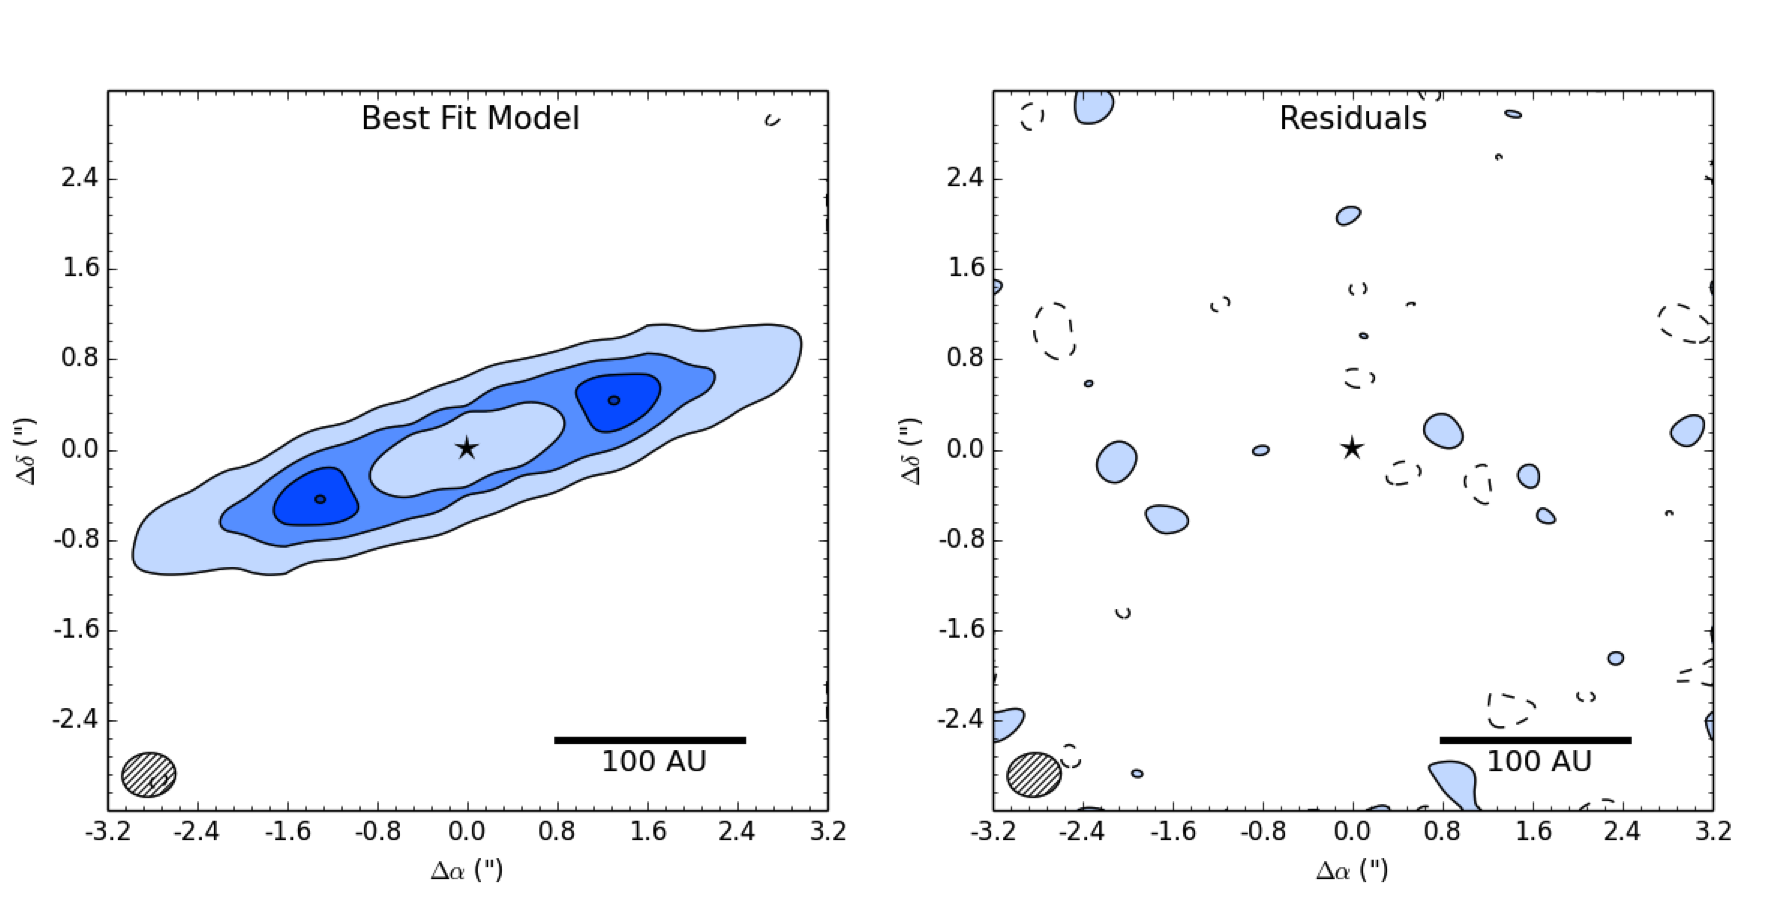
\includegraphics[width = 1\textwidth]{49CET_nOBAG_ModelResidual.png}
\caption{The model image (left) and residuals (right) for the single power law model with two characteristic grain sizes. Contours are [-2, 2, 4, 6, 8] $\times$ 58$\,\mu$Jy.}
\label{fig:49CET_nOBAG_ModelResidual}
\end{figure}

Given the success of the single power law description of the surface density fitting just the visibilities but the discrepancies introduced in a simultaneous fit, we propose an inner disk of grains, with a different characterization of the surface density, is necessary to recreate the mid-IR excess. Building upon the results of \cite{Wahh07}, who resolved the inner disk of small grains and had a best fit model that specified $a$ = 0.1$\,\mu m$, we described an inner disk with a grain size of 0.1$\,\mu m$ from $R_{In}$ to $R_{Inner Disk}$ with $\Sigma_{Inner Disk} \propto r^{-1}$, and vary all the parameters described by Equation \ref{eq:sigma100} as an outer belt, which extends from $R_{Inner Disk}$ to $R_{Out}$. The outer radius of the disk is modeled as $R_{In}$ + $\Delta R$. Because small grains radiate at higher temperatures at a given distance from the star than their larger brethren as described by \ref{eq:fullEBalance}, they were able to boost the mid-IR flux without contributing significantly to the flux at millimeter wavelengths.


\begin{figure}%[!]
\centering
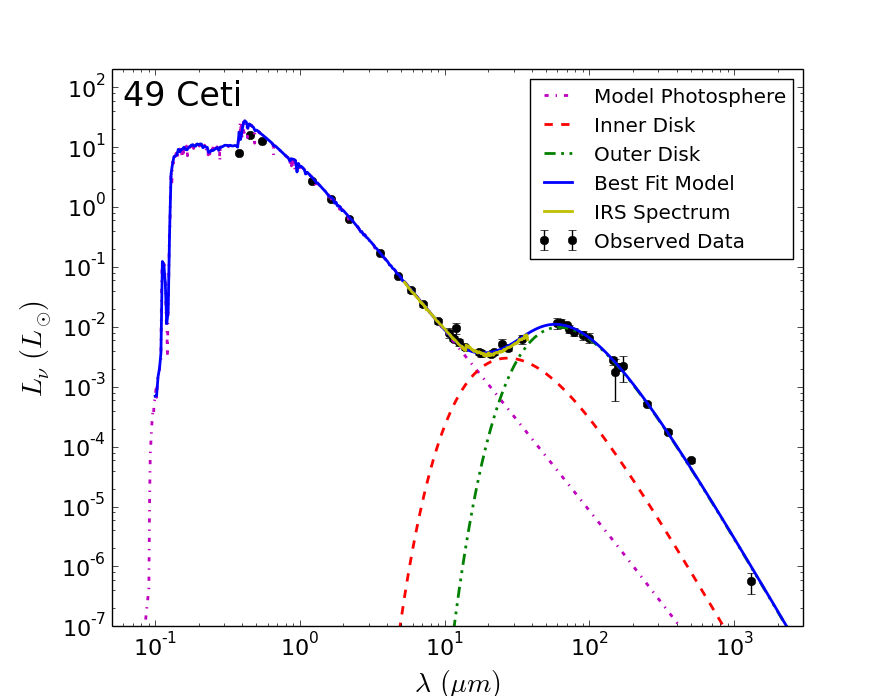
\includegraphics[width = 1\textwidth]{49CET_nOBAG_SED.png}
\caption{The best fit SED of 49 Ceti for the single power law model simultaneously fitting the SED and visibilities with two characteristic grain sizes. The best fit model is the sum of the inner disk model, outer disk model, and the model photosphere.}
\label{fig:49CET_nOBAG_SED}
\end{figure}

\begin{table}
\begin{center}
    \def\arraystretch{1.1}%
    \begin{tabular}{l*{2}{c}r}
    \hline
    Parameter & Median Value $\pm$ 1$\sigma$ & Best Fit Value \\ \hline
     $R_{In}$  [AU] & 5$^{+2}_{-1}$ & 6\\  
     $R_{Inner Disk}$ [AU] & 73$^{+3}_{-3}$ & 73\\      
     $\Delta R$ [AU] & 310$^{+9}_{-9}$ & 310\\ 
     log($M_{Outer Disk}$ [$M_{\oplus}$]) & -1.17$^{+0.08}_{-0.10}$ & -1.16 \\
     log($M_{Inner Disk}$ [$M_{M_{\oplus}}$]) & -3.1$^{+0.2}_{-0.2}$ & -3.0 \\     
     log(a [$\mu$m]) & 0.08$^{+0.11}_{-0.14}$ & 0.09\\ 
     $\beta$ & 1.17$^{+0.05}_{-0.05}$ & 1.18\\ 
     $p$ & 1.29$^{+0.11}_{-0.11}$ & 1.27\\ 
     $i$ [$^\circ$] & 79.4$^{+0.4}_{-0.4}$ & 79.3 \\ 
     $PA$ [$^\circ$] & -71.4$^{+0.4}_{-0.5}$ & -71.3\\
    \hline
    \end{tabular}
\end{center}
\caption{The median and best fit values for the single power law model with two characteristic grain sizes simultaneously fitting the SED and visibilities.}
\label{tab:49CET_nOBAG_Table}
%for all parameters of the model of 49 Ceti's dust disk. THIS IS SIMPLE BONUS BELT, JUST VIS100x840}
\end{table}


%%%%%%%

\section{The Unresolved Surface Density Enhancement (USDE)}
\label{USDE}

\subsection{Visibility-only Fit}
\label{USDE_Vis}

\begin{figure}[t!]
\centering
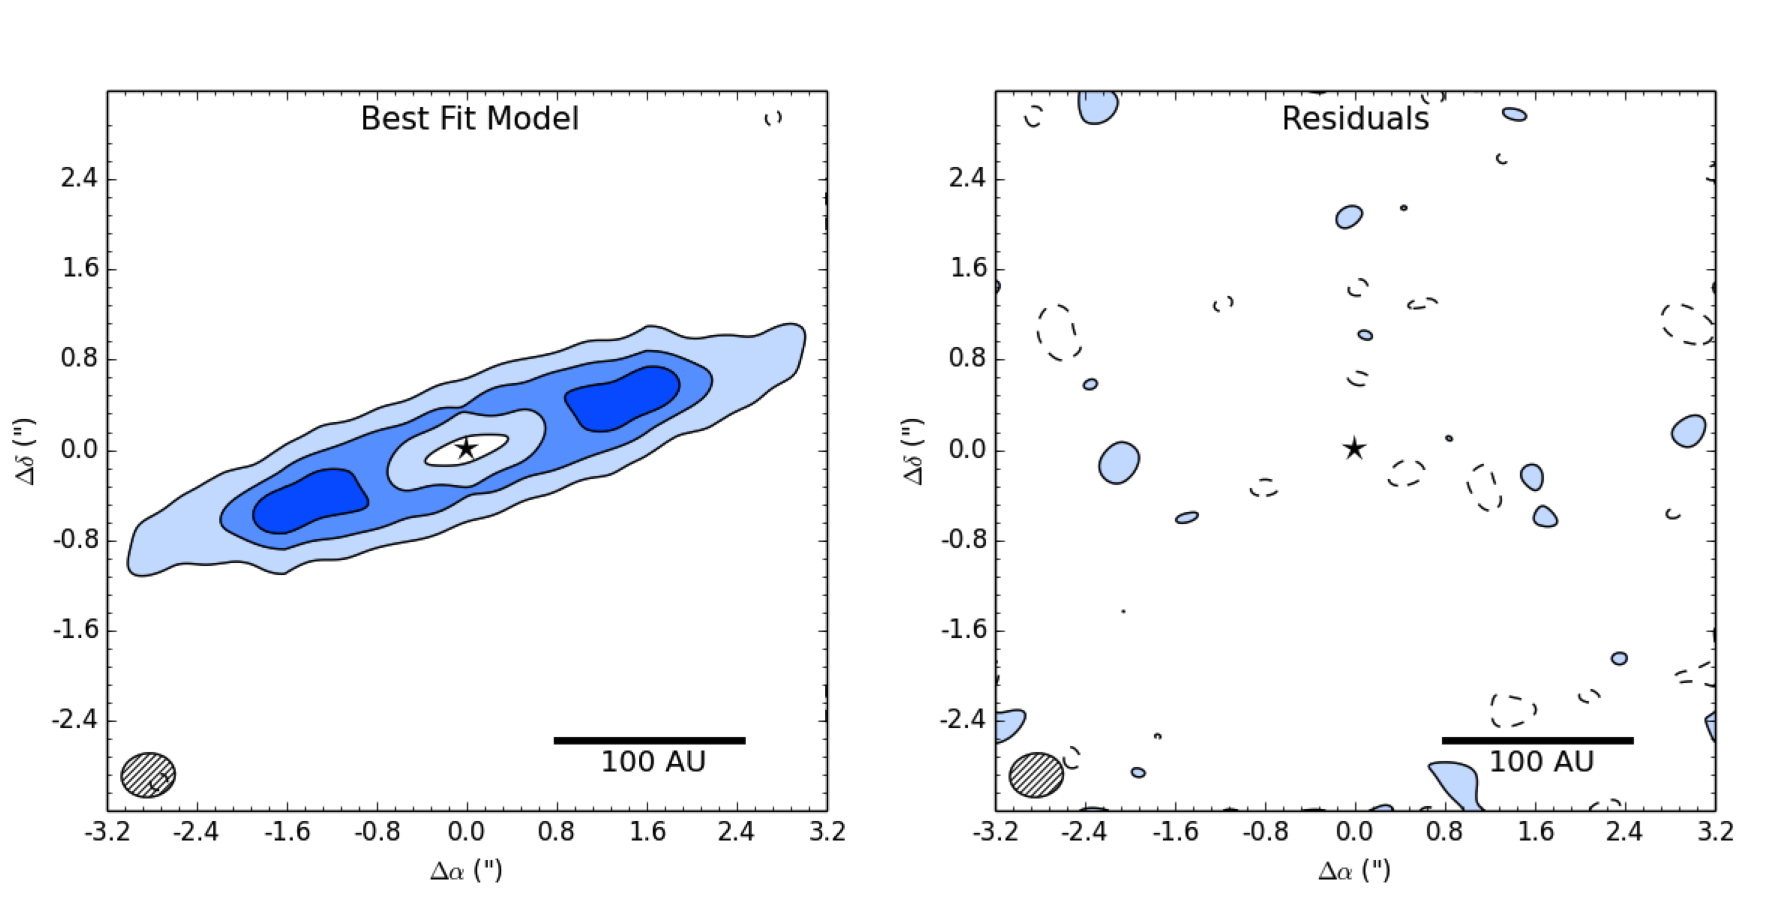
\includegraphics[width = 1\textwidth]{49CET_BonusBeltVIS_ModelResidual.png}
\caption{The model image (left) and residuals (right) for the unresolved surface density enhancement model fitting just the visibilities. Contours are [-2, 2, 4, 6] $\times$ 58$\,\mu$Jy. The model leaves only a small scatter of 2$\sigma$ residuals.}
\label{fig:49CET_BonusBeltVIS_ModelResidual}
\end{figure}

Although the single power law description of the surface density adequately describes the data, the ring-like structure apparent at $\sim$ 100\,AU in the data image suggests a ring-like description of the surface density in our model could provide a better fit. To do this, we add a narrow, spatially unresolved belt, which we model to be 3\,AU wide at a distance $R_{Belt}$ and of mass $M_{Belt}$, on top of of the single power law description of the surface density that extends from $R_{In}$ to $R_{Out}$ as described in Section \ref{SinglePowerSED_Model}. 

As can be seen in the best-fit model and residual images displayed in Figure \ref{fig:49CET_BonusBeltVIS_ModelResidual}, this USDE model does a very good job of recreating the visibilities, and the residual image seems identical to that of the single power law visibility-only fit (see Section \ref{stats} for the statistical analysis of the comparison between these fits). Both models show evidence for an inner disk that is devoid of large grains, as the best-fit inner radius of 56\,AU derived in this model is close to the value of 69\,AU derived in the single power law visibility-only fit (see Table \ref{tab:49CET_BonusBeltVIS_Table} for all parameters derived from the MCMC chain for this model). 


%However, 49 Ceti seems to show a ring-like structure at $\sim$ 100 AU, suggesting a more complex model of the surface density could provide a better fit. A simple power law with a narrow density enhancement to mimic this ``ring" is described in Section ??<<??, and a double power law, with surface density increasing to the radius of this ``ring" before decreasing, is presented in Section ??<<??????. 

%The ring-like positive residuals left by the single power law model suggest the need for a more complex model of the surface density. We propose a double power law model in which the surface density increases from $R_{In}$ to a transition radius $R_{T}$ before dropping off until $R_{Out}$ in section \ref{DoublePowerSED_Model} and a single power law with a narrow, unresolved surface density enhancement in section \ref{UnresolvedDensitySED_Model}.

%Unlike the double power law model, fitting to just the visibilities with the best-fit unresolved density enhancement model resolves the inner radius of the disk to be 56AU (See Table \ref{tab:49CET_BonusBeltVIS_Table}), whereas the double power law model settled on a best-fit of 6AU. This larger value for $R_{In}$ is visible in the best-fit model image (Figure \ref{fig:49CET_BonusBeltVIS_ModelResidual}), as there is no emission next to the star. However, this difference has no significant effect on the residual image map, which shows basically the same scatter of -2$\sigma$ residuals as in the double power law best-fit residual image. 

%To see how strongly the SED was altering the best-fit models, we ran fits with MCMC based just on the visibility $\chi^{2}$. We find that both the double power law and unresolved surface density enhancement models are able to recreate the visibilities, and that differences between parameters between the two models are not significant. This is clear both from the minimal leftovers in each residual image and from an F-test, which confirmed that neither model is better the other in a statistically significant way.

%Both models settle on approximately the same radius for the peak of the surface density. $R_{T}$ = 105AU for the double power law model, and $R_{Belt}$ = 113AU for the unresolved surface density enhancement model. Without the simultaneous fit to the SED, $M_{Disk}$, $\beta$, and $a$ are not well constrained.

\begin{table}
\begin{center}
    \def\arraystretch{1.37}%
    \begin{tabular}{l*{2}{c}r}
    \hline
    Parameter & Median Value $\pm$ 1$\sigma$ & Best Fit Value \\ \hline
     $R_{In}$  [AU] & 58$^{+6}_{-6}$ & 56\\  
     $\Delta R$ [AU] & 248$^{+8}_{-8}$ & 252\\ 
     log($M_{Disk}$ [$M_{\oplus}$]) & -0.8$^{+0.5}_{-0.9}$ & -0.7 \\
     $R_{Belt}$  [AU] & 114$^{+3}_{-3}$ & 113\\ 
     log($M_{Belt}$ [$M_{\oplus}$]) & -1.9$^{+0.6}_{-0.8}$ & -1.6\\
     log(a [$\mu$m]) & 0.3$^{+0.9}_{-0.7}$ & -0.1\\ 
     $\beta$ & 1.4$^{+0.4}_{-0.4}$ & 1.4\\ 
     $p$ & 0.6$^{+0.4}_{-0.4}$ & 0.6\\ 
     $i$ [$^\circ$] & 79.4$^{+0.4}_{-0.4}$ & 79.4 \\ 
     $PA$ [$^\circ$] & -71.2$^{+0.4}_{-0.6}$ & -71.1\\
    \hline
    \end{tabular}
\end{center}
\caption{The median and best fit values for the unresolved density enhancement model fitting only the visibilities.}
\label{tab:49CET_BonusBeltVIS_Table}
%for all parameters of the model of 49 Ceti's dust disk. THIS IS SIMPLE BONUS BELT, JUST VIS100x840}
\end{table}


\subsection{Simultaneous SED and Visibility Fit}

Simultaneously fitting the USDE model to the SED and visibilities comes close to recreating both the images and the visibilities, but runs into similar issues that the single power law model of Section \ref{Simple_SED_Vis} encountered. The sum of the fluxes from the model photosphere, broad power law disk, and narrow ring is displayed in Figure \ref{fig:49CET_BonusBeltSED_SED} and is a good fit to the photometric data. While the IR excess is dominated by the disk model, the belt contributes a non-negligible flux to the SED, both at the IR excess peak of $\sim$ 70$\,\mu m$ and at the wavelength of the ALMA image (850$\,\mu m$). 

\begin{figure}%[t!]
\label{fig:49CET_BonusBeltSED_SED}
\centering
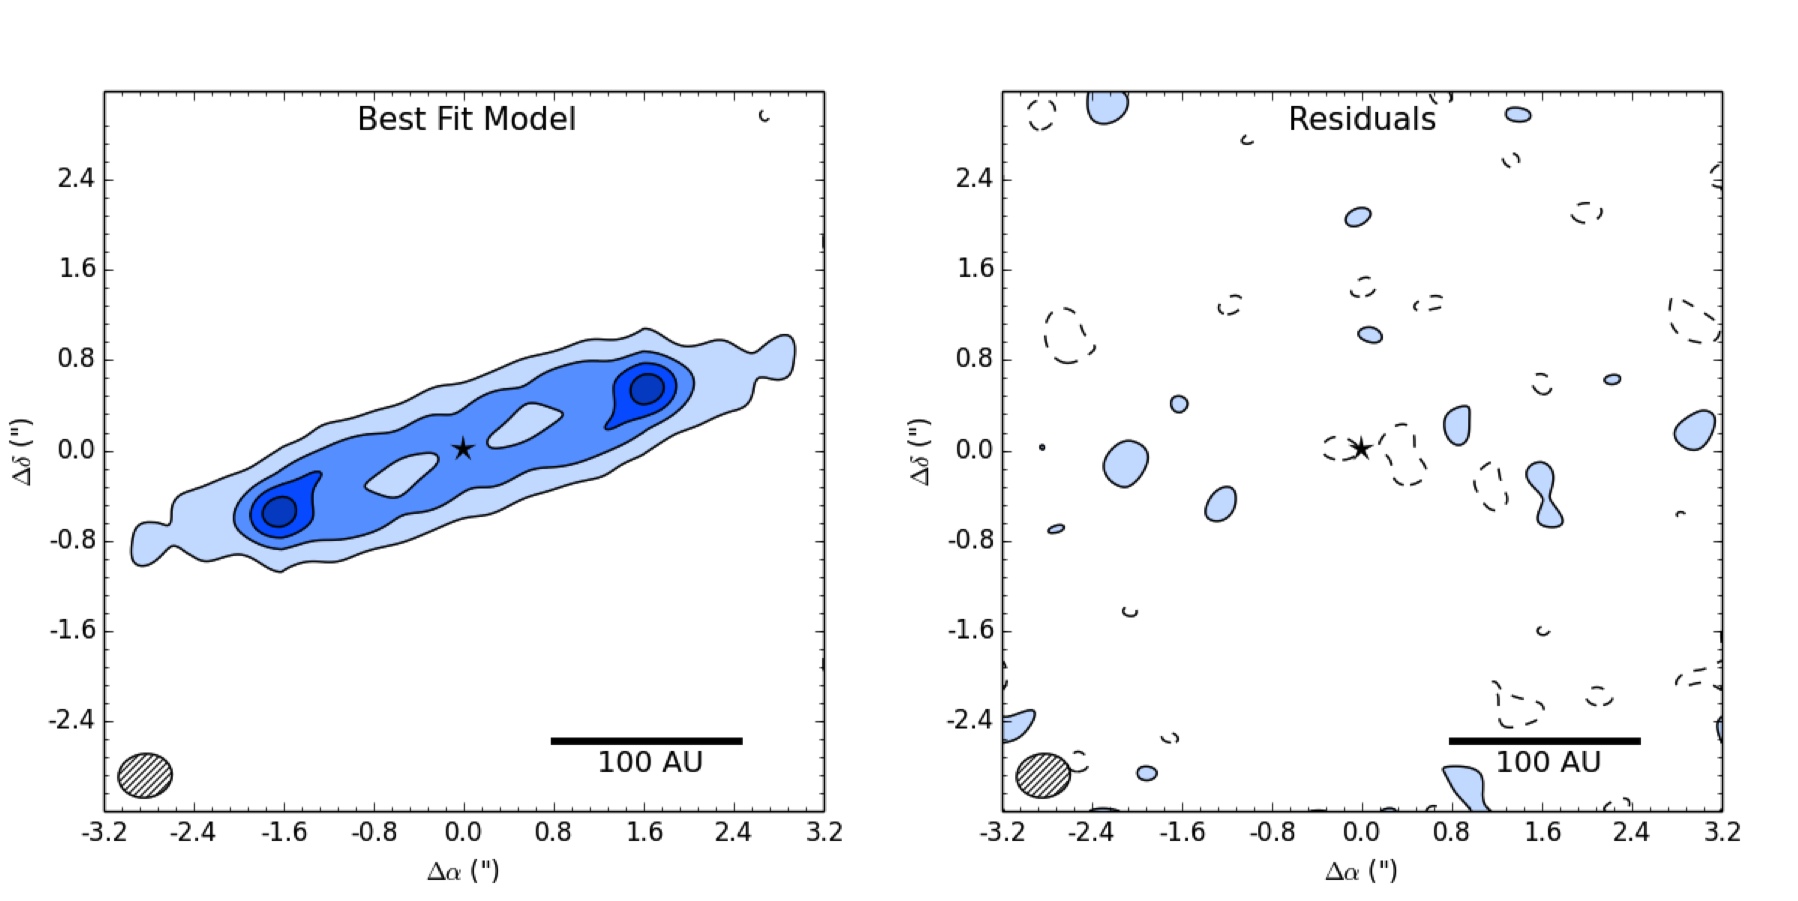
\includegraphics[width = 1\textwidth]{49CET_BonusBeltSED_ModelResidual.png}
\caption{The model image (left) and residuals (right) for the unresolved surface density enhancement model, simultaneously fitting the SED and the visibilities. Contours are [-2, 2, 4, 6, 8] $\times$ 58$\,\mu$Jy. The model successfully takes care of the region of high density on the southeast side of the disk, but is still slightly too bright at the center.}
\label{fig:49CET_BonusBeltSED_ModelResidual}
\end{figure}

\begin{figure}%[H]
\centering
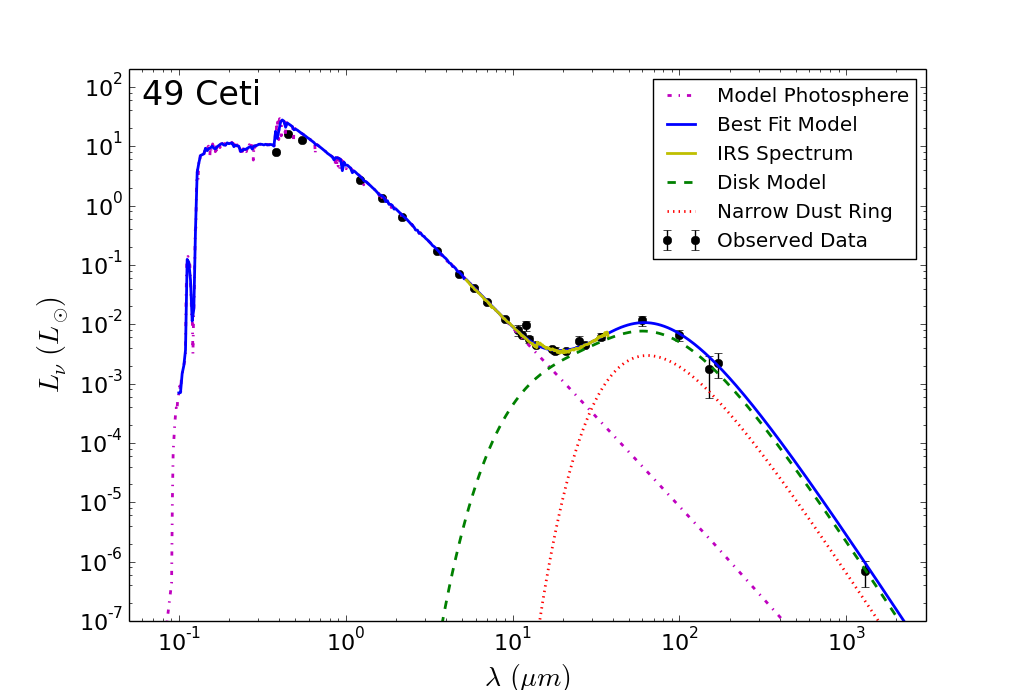
\includegraphics[width = 1\textwidth]{49CET_BonusBeltSED_SED.png}
\caption{The best fit SED of 49 Ceti for the unresolved surface density enhancement model. The best fit model is the sum of the disk model, the model photosphere, and the narrow dust ring.}
\label{fig:49CET_BonusBeltSED_SED}
\end{figure}

\begin{table}
\begin{center}
    \def\arraystretch{1.2}%
    \begin{tabular}{l*{2}{c}r}
    \hline
    Parameter & Median Value $\pm$ 1$\sigma$ & Best Fit Value \\ \hline
     $R_{In}$  [AU] & 1.3$^{+0.7}_{-0.5}$ & 1.3\\  
     $\Delta R$ [AU] & 290$^{+8}_{-7}$ & 291\\ 
     log($M_{Disk}$ [$M_{\oplus}$]) & -1.1$^{+0.2}_{-0.2}$ & -1.1 \\
     $R_{Belt}$  [AU] & 112$^{+2}_{-2}$ & 112\\ 
     log($M_{Belt}$ [$M_{\oplus}$]) & -1.8$^{+0.2}_{-0.2}$ & -1.7\\
     log(a [$\mu$m]) & 0.27$^{+0.17}_{-0.19}$ & 0.31\\ 
     $\beta$ & 1.25$^{+0.15}_{-0.12}$ & 1.27\\ 
     $p$ & -0.11$^{+0.06}_{-0.06}$ & -0.07\\ 
     $i$ [$^\circ$] & 79.5$^{+0.4}_{-0.4}$ & 79.5 \\ 
     $PA$ [$^\circ$] & -71.0$^{+0.4}_{-0.4}$ & -71.0\\
    \hline
    \end{tabular}
\end{center}
\caption{The median and best fit values for the unresolved density enhancement model fitting the SED and visibilities.}
%for all parameters of the model of 49 Ceti's dust disk. THIS IS SIMPLE BONUS BELT, VIS & SED 120x842 WITH CORRECT UNCERTAINTIES}
\label{tab:49CET_BonusBeltSED_Table}
\end{table}

However, the simultaneous best-fit USDE model has $R_{In}$ = 1.3\,AU in order to generate enough hot grains to recreate the mid-IR excess of the SED, and with just one characteristic grain size ($a \sim 2\,\mu m$), the inner disk contributes too much flux at the wavelength of the ALMA image. This results in more in negative residuals than were apparent in the visibility-only fit at the center of the best-fit residual image as can be seen in Figure \ref{fig:49CET_BonusBeltSED_ModelResidual}. This model suggests a surface density that increases slightly with radius ($p$ = $-0.07$), but the visibility-only fit found $p$ = 0.6, showing that the SED's influence is resulting in an inferior fit to the visibilities. Because of the addition of the unresolved density enhancement, this model does better at accounting for the ring-like residuals that were left behind by the single power law model with one characteristic grain size, but as with the single power law, the discrepancy between the visibility-only fit and the simultaneous fit necessitates a disk model with two characteristic grain sizes. 


%The best-fit model and residuals are displayed in Figure \ref{fig:49CET_BonusBeltSED_ModelResidual}, and the table of values derived from the MCMC chain is presented in Table \ref{tab:49CET_BonusBeltSED_Table}. The best-fit SED is shown in Figure \ref{fig:49CET_BonusBeltSED_SED}, with separate contributions to the total flux of the model displayed for the broad disk described by the single power law and by the additional belt. 

%The total best-fit mass for this model is 0.10 $M_{\oplus}$, whereas the simple power law model had a mass of 0.23$M_{\oplus}$
%The best-fit value of $p$ shows that the disk is nearly flat, whereas
%This model does a better job at recreating the density enhancement in the disk and still fitting to the SED, but just like with the double power law model, it is too bright at the center. As earlier, in order to create grains hot enough to boost the mid-IR flux with only one characteristic grain size population, the inner radius of the disk is pushed inward to ~1AU. These grains are then able to recreate the mid-IR excess, but in doing so contribute too much flux at the wavelength of the ALMA image, resulting in a model that is too bright near the star.

\subsection{Simultaneous SED and Visibility Fit with Two Characteristic Grain Sizes}

\begin{figure}[t!]
\centering
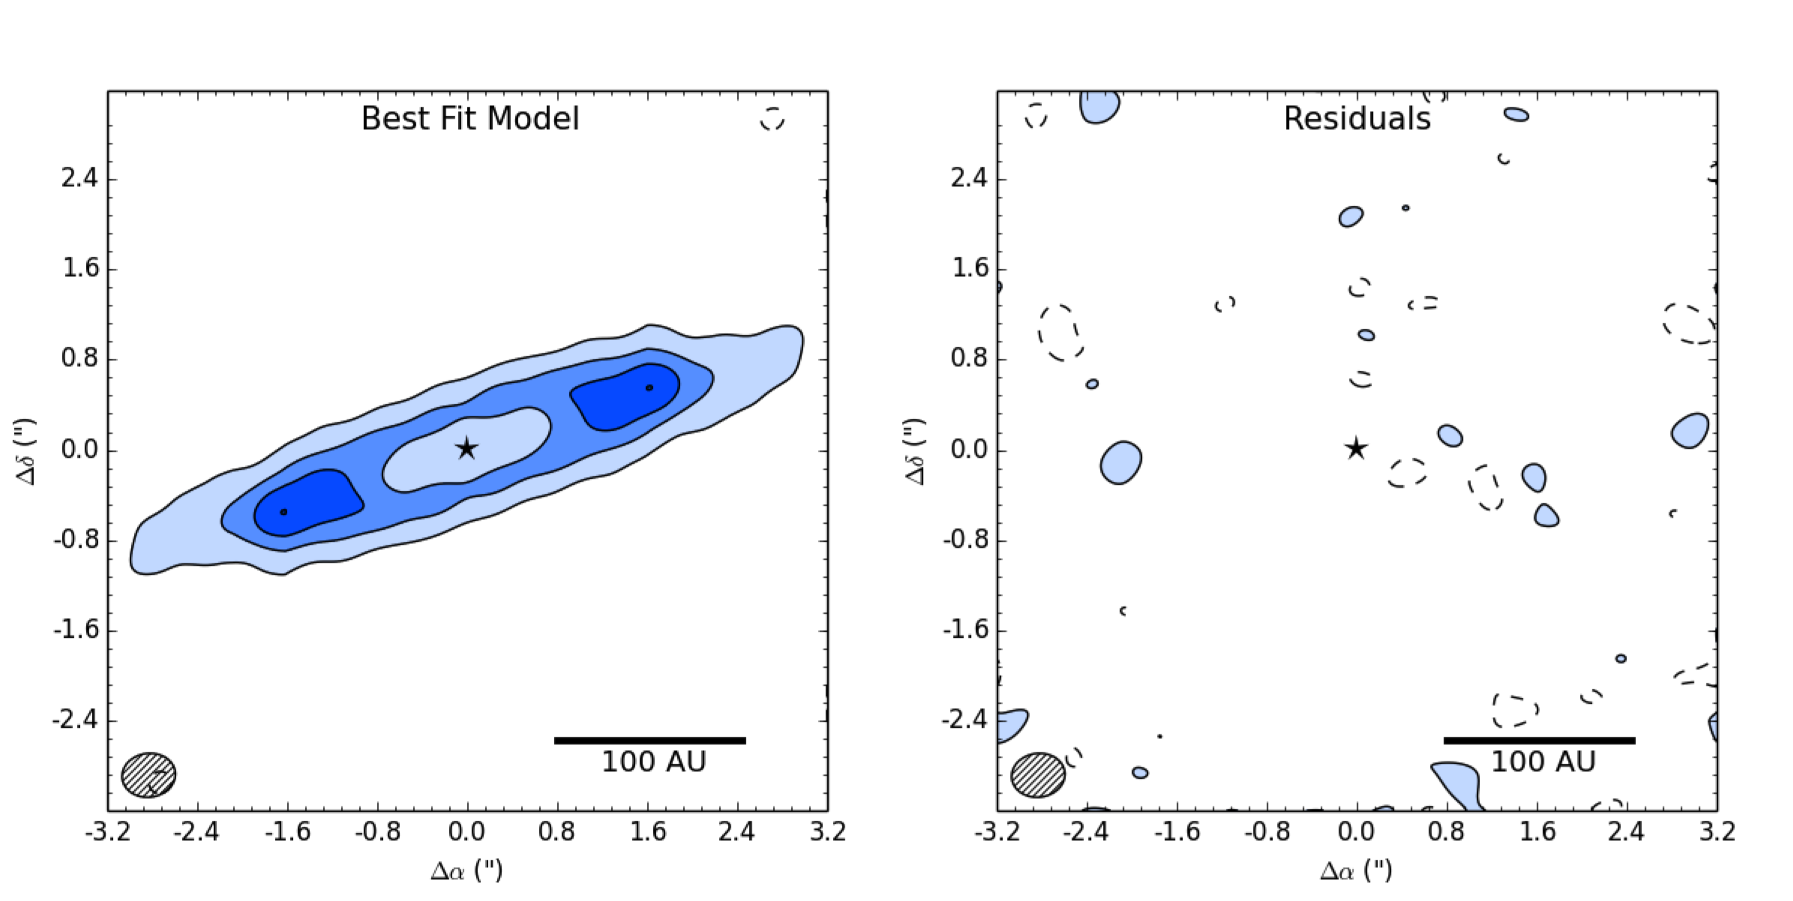
\includegraphics[width = 1\textwidth]{49CET_bBBAG_ModelResidual.png}
\caption{The model image (left) and residuals (right) for the USDE model with an an additional inner disk of small grains. Contours are [-2, 2, 4, 6, 8] $\times$ 58$\,\mu$Jy. The model leaves only a small scatter of 2$\sigma$ residuals.}
\label{fig:49CET_bBBAG_ModelResidual}
\end{figure}
\end{table}

As earlier, we implement an inner disk of 0.1$\,\mu m$ grains from $R_{In}$ to $R_{Inner Disk}$ with $\Sigma_{Inner Disk} \propto r^{-1}$ to complement the outer disk with the additional surface density enhancement described above. This model is able to simultaneously fit the SED (not displayed) without it significantly influencing the best-fit parameters derived from the USDE visibility-only fit (Section \ref{USDE_Vis}). For example, the best-fit value of $p$ derived in the USDE model with two characteristic grain sizes is 0.75, which is statistically equivalent to that of the USDE visibility-only best-fit value within our uncertainties (see Table \ref{tab:bBBAG_Table}). Both this model and the single power law with two characteristic grain sizes settle on $R_{Inner Disk} \sim$ 70\,AU, providing further evidence that there is a clear turnover around this radius of an inner disk of small grains and an outer disk of larger grains. The best-fit model and residuals are displayed in Figure \ref{fig:49CET_bBBAG_ModelResidual} and look very similar to those of the single power law model with two characteristic grain sizes, though the peak of $8\sigma$ emission apparent in this model is farther out than in the other model, a result of the surface density peaking at $\sim$ 114\,AU rather than $\sim$ 73\,AU. 

\begin{figure}%[t!]
\label{fig:49CET_USDE_TWO_SED}
\centering
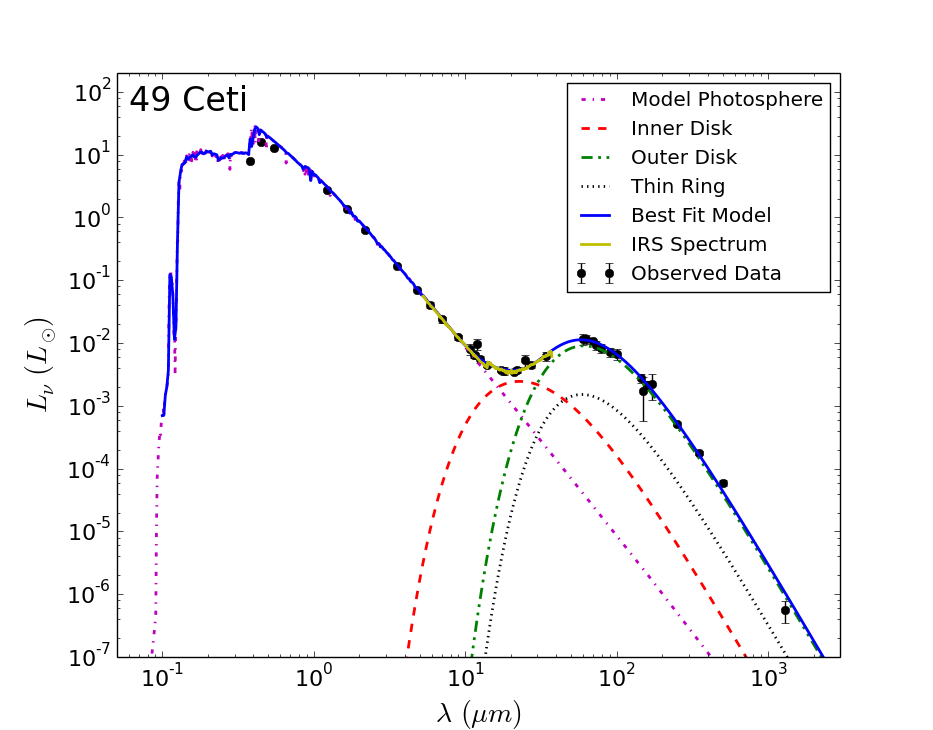
\includegraphics[width = \textwidth]{49CET_bBBAG_SED.png}
\caption{The SED for the USDE model fitting the SED and visibilities for the two part disk model. The best fit model is the sum of the inner disk, outer disk, narrow ring, and model photosphere. }
\label{fig:49CET_BonusBeltSED_ModelResidual}
\end{figure}



\begin{table}
\begin{center}
    \def\arraystretch{1.2}%
    \begin{tabular}{l*{2}{c}r}
    \hline
    Parameter & Median Value $\pm$ 1$\sigma$ & Best Fit Value \\ \hline
     $R_{In}$  [AU] & 4.6$^{+1.5}_{-1.2}$ & 3.5\\  
     $\Delta R_{Out}$ [AU] & 302$^{+9}_{-8}$ & 303\\ 
     $R_{Inner Disk}$ [AU] & 62$^{+5}_{-5}$ & 60\\ 
     $R_{Ring}$  [AU] & 114$^{+3}_{-3}$ & 114\\ 
     log($M_{Inner Disk}$ [$M_{\oplus}$]) & -3.3$^{+0.2}_{-0.2}$ & -3.4 \\
     log($M_{Outer Disk}$ [$M_{\oplus}$]) & -1.21$^{+0.09}_{-0.10}$ &-1.21 \\
     log($M_{Ring}$ [$M_{\oplus}$]) & -2.26$^{+0.15}_{-0.18}$ &-2.26 \\
     log(a [$\mu$m]) & 0.09$^{+0.10}_{-0.13}$ & 0.06\\ 
     $\beta$ & 1.17$^{+0.05}_{-0.05}$ & 1.17\\ 
     $p$ & 0.80$^{+0.19}_{-0.17}$ & 0.75\\ 
     $i$ [$^\circ$] & 79.3$^{+0.4}_{-0.4}$ & 79.3 \\ 
     $PA$ [$^\circ$] & -71.4$^{+0.4}_{-0.4}$ & -71.2\\
    \hline
    \end{tabular}
\end{center}
\caption{Parameters derived from the MCMC chain for the USDE model with two characteristic grain sizes.}
\label{tab:bBBAG_Table}
\end{table}


%%%%%%%%%%%%%%%%%%%%%%%%%

\section{The Double Power Law}
\label{DP}

Another means of describing a ring-like structure is with a double power law that increases in surface density to a variable radius before dropping off. This model, which has the same number of free parameters as the USDE model, provides a comparison for us to discern whether or not the surface density enhancement is resolved in our data. We parameterize $\Sigma(r)$ for the double power law normalized to the surface density at the transition radius, $\Sigma_{T}$. We model the transition radius, $R_{T}$ as $R_{In} + \Delta R_{T}$, and the outer radius, $R_{Out}$, as $R_{In} + \Delta R_{T} + \Delta R_{Out}$.

\begin{equation}\label{eq:sigmaDP}
\Sigma(r) = \begin{cases}
   \Sigma_{T}\Big(\frac{r}{R_{T}}\Big)^{-p_{1}} & \text{for $R_{In}$ $\le$ r $\le R_{T}$} \\
   \Sigma_{T}\Big(\frac{r}{R_{T}}\Big)^{-p_{2}} & \text{for $R_{T}$ $\textless$ r $\le$ $R_{Out}$}
\end{cases}
\end{equation}

As earlier, we solve for $M_{Disk}$:

\begin{equation}\label{eq:mdiskDP}
\begin{flalign*}
    M_{Disk} &= \int_{R_{In}}^{R_{T}} \Sigma(r) 2 \pi r \,dr & \\
    &= \int_{R_{In}}^{R_{T}} \Sigma_{\text{T}}\Big(\frac{r}{R_{T}}\Big)^{-p_{1}} 2 \pi r \,dr & + \int_{R_{T}}^{R_{Out}} \Sigma_{\text{T}}\Big(\frac{r}{R_{T}}\Big)^{-p_{2}} 2 \pi r \,dr &&
\end{flalign*}
\end{equation}

We integrate and solve for $\Sigma_{T}$, defining $j_{1} = 2 - p_{1}$, $j_{2} = 2 - p_{2}$, $m_{1} = R_{T}^{j_{1}} - R_{In}^{j_{1}$, and $m_{2} = R_{Out}^{j_{2}} - R_{T}^{j_{2}$ for readability:

\begin{equation}\label{eq:sigmaT}
\Sigma_{T} = \cfrac{M_{Disk} (j_{1} j_{2})}{2\pi [(m_{1} j_{2})(R_{T})^{p_{1}} + (m_{2} j_{1})(R_{T})^{p_{2}}]}
\end{equation}

This parameterization of $\Sigma_{T}$ allows us to vary $R_{In}$, $R_{T}$, $R_{Out}$, $M_{Disk}$, $p_{1}$, and $p_2$ in our search for a best-fit model. We use $a$ and $\beta$ to describe the population of grains and $i$ and $PA$ to describe the geometry on the sky as in the single power law model. 

\subsection{Visibility-only Fit}

\begin{figure}
\centering
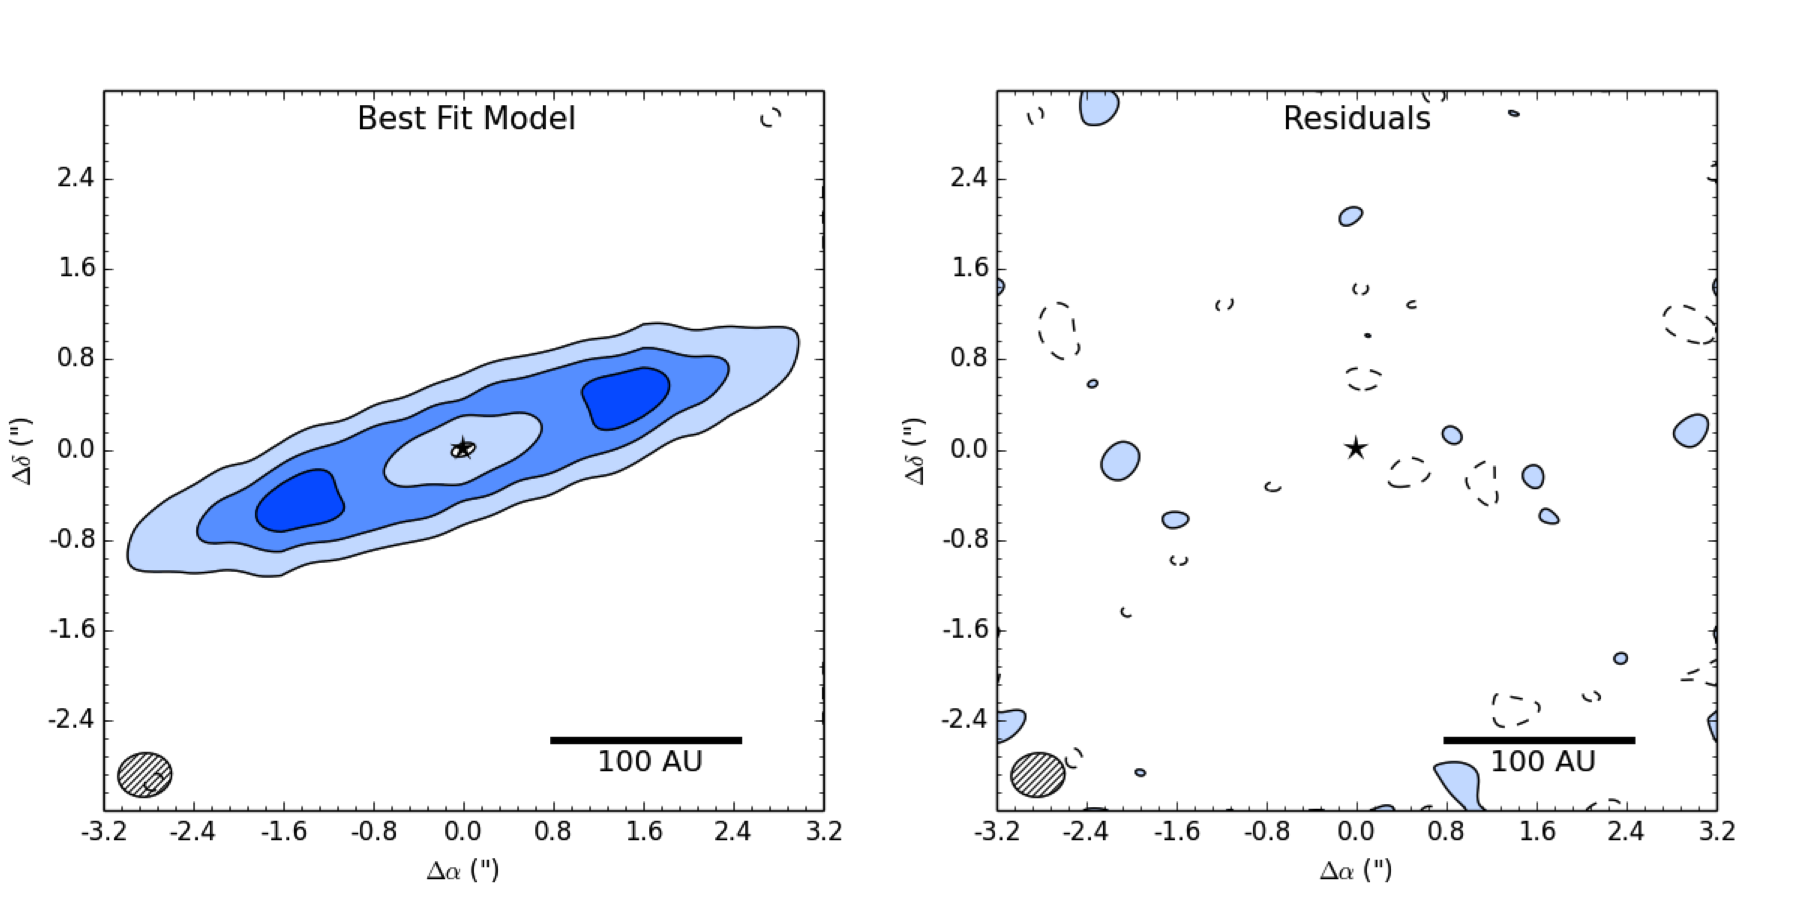
\includegraphics[width = 1\textwidth]{49CET_DoublePowerVIS_ModelResidual.png}
\caption{The model image (left) and residuals (right) for the double power law model fitting just the visibilities. Contours are [-2, 2, 4, 6] $\times$ 58$\,\mu$Jy. The model leaves only a small scatter of 2$\sigma$ residuals.}
\label{fig:49CET_DoublePowerVIS_ModelResidual}
\end{figure}

\begin{table}
\begin{center}
    \def\arraystretch{1.37}%
    \begin{tabular}{l*{2}{c}r}
    \hline
    Parameter & Median Value $\pm$ 1$\sigma$ & Best Fit Value \\ \hline
     $R_{In}$  [AU] & 26$^{+20}_{-17}$ & 6\\  
     $\Delta R_{T}$ [AU] & 78$^{+16}_{-17}$ & 99\\ 
     $\Delta R_{Out}$ [AU] & 215$^{+13}_{-12}$ & 212\\ 
     log($M_{Disk}$ [$M_{\oplus}$]) & -1.4$^{+0.5}_{-0.5}$ & -2.2 \\
     log(a [$\mu$m]) & 0.5$^{+0.4}_{-0.4}$ & 0.4\\ 
     $\beta$ & 1.4$^{+0.3}_{-0.3}$ & 0.8\\ 
     $p1$ & -1.7$^{+0.6}_{-0.6}$ & -1.8\\ 
     $p2$ & 1.52$^{+0.19}_{-0.16}$ & 1.55\\ 
     $i$ [$^\circ$] & 79.2$^{+0.4}_{-0.4}$ & 79.1 \\ 
     $PA$ [$^\circ$] & -71.7$^{+0.5}_{-0.5}$ & -71.5\\
    \hline
    \end{tabular}
\end{center}
\caption{The median and best fit values for the double power law model fitting only the visibilities.}
% for all parameters of the model of 49 Ceti's dust disk, THIS IS DOUBLE POWER VIS ONLY 100x600}
\label{tab:49CET_DoublePowerVIS_Table}
\end{table}

Fitting to just the visibilities with the double power law model adequately describes the data, as can be seen by the lack of significant residuals in Figure \ref{fig:49CET_DoublePowerVIS_ModelResidual}. The values derived from the MCMC chain are displayed in Table \ref{tab:49CET_DoublePowerVIS_Table}. Although the best-fit inner radius of this model is still close to the star ($\sim$ 6\,AU), it ramps up toward $R_{T}$ quite steeply ($\Sigma_{Inner Disk} \propto r^{1.8}$) and doesn't result in any systematic -2$\sigma$ residuals near the star. In addition, not under the influence of the SED, it is able to recreate the region of higher density. 

\subsection{Simultaneous SED and Visibility Fit}

\begin{figure}
\centering
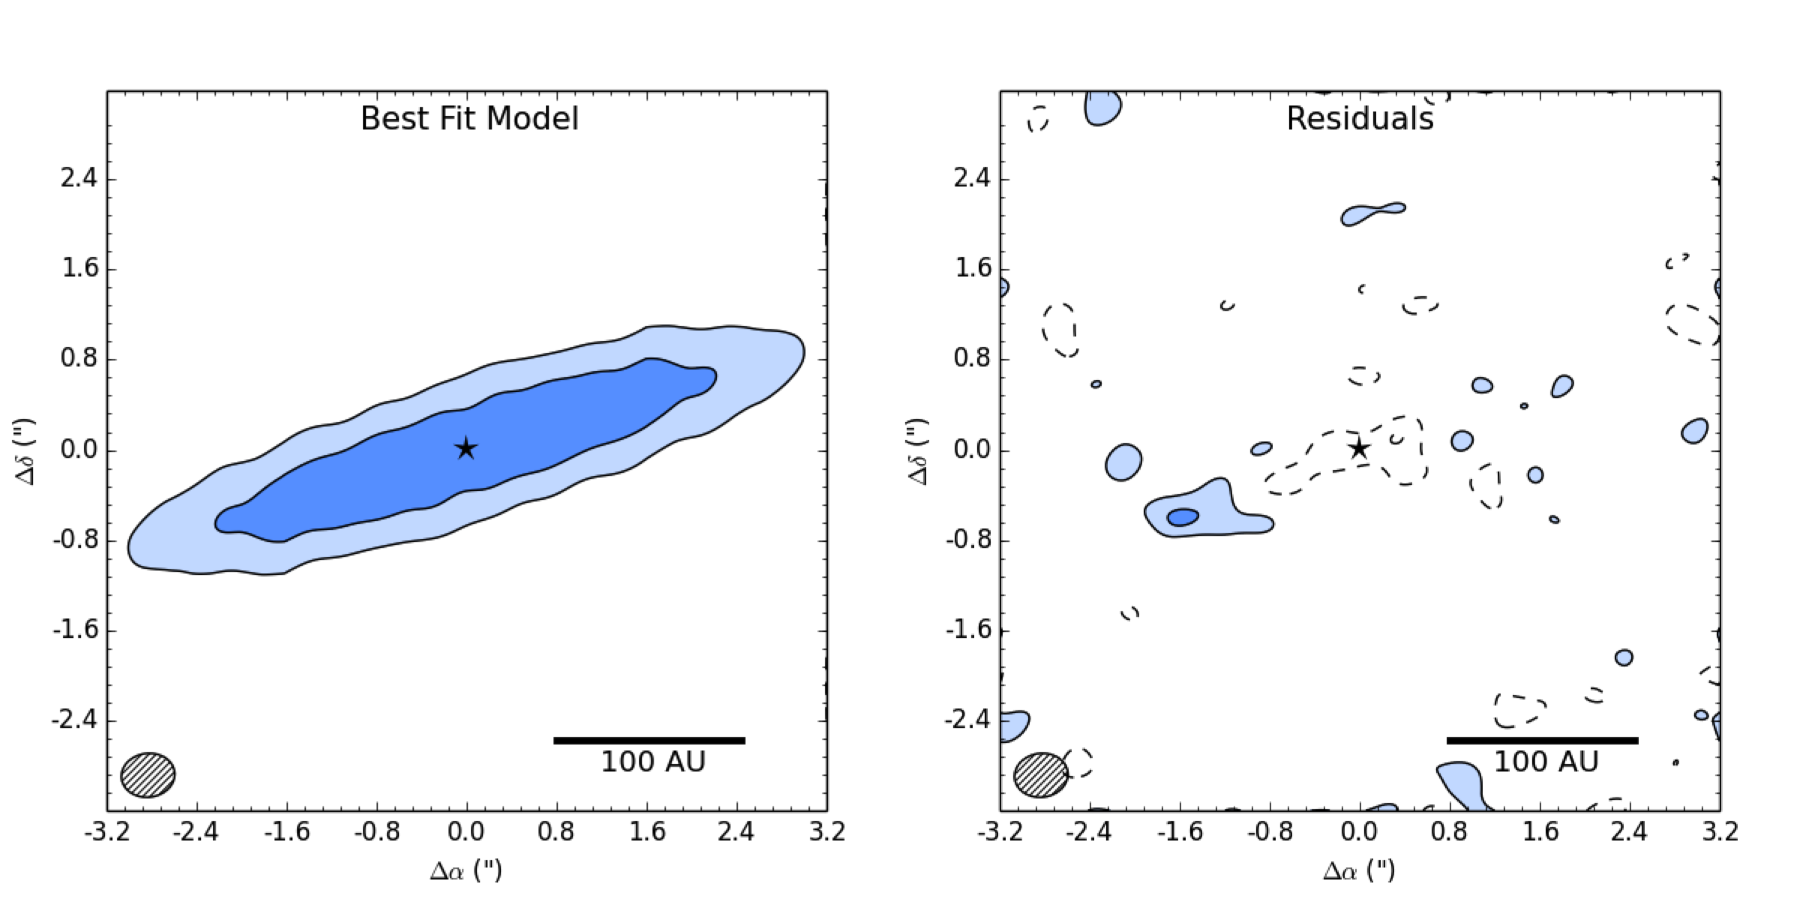
\includegraphics[width = 1\textwidth]{49CET_DoublePowerSED_ModelResidual.png}
\caption{The model image (left) and residuals (right) for the double power law model, simultaneously fitting the SED and the visibilities. Contours are [-4, -2, 2, 4] $\times$ 58$\,\mu$Jy.}
\label{fig:49CET_DoublePowerSED_ModelResidual}
\end{figure}

Values derived from the MCMC chain for the double power law model simultaneously fitting to the SED and visibilities are presented in Table \ref{tab:doublePowerSEDTable}, and the best-fit model and corresponding residuals are displayed in Figure \ref{fig:49CET_DoublePowerSED_ModelResidual}. This model returned a best-fit value for $p_{1}$ of $-$0.25, which is significantly different from that derived in the visibility-only fit ($p_{1} = -1.8$), resulting in a disk model that is too bright at small radii. In addition, the model was unable to account for the region of higher density on the southeast side apparent in the resolved ALMA data, even though it was able to in the visibility-only fit. As with earlier simultaneous fits with just one characteristic grain size, these effects are the result of the fit to the SED (Figure \ref{fig:49CET_DP_SED}). 

\begin{figure}%[t!]
\label{fig:49CET_DP_SED}
\centering
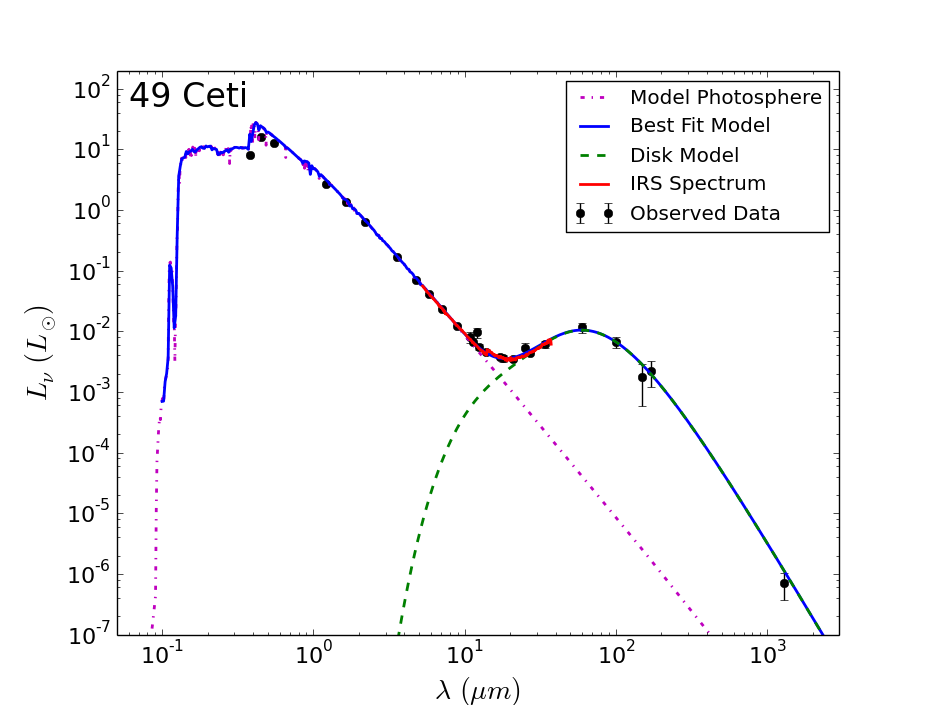
\includegraphics[width = 1\textwidth]{49CET_DP_SED.png}
\caption{The SED for the double power law model fitting the SED and visibilities for the disk model with just one characteristic grain size. }
\label{fig:49CET_DP_SED}
\end{figure}

%In addition, it is brighter at the center of the disk than even the simple power law model, as can be seen from the larger area of -2$\sigma$ residuals near the star. However, this model succeeds at getting rid of much of the ring-like 2$\sigma$ residuals left by the single power law model.

%The double power law model's attempt to simultaneously recreate the SED and visibilities forces $R_{In}$ to smaller radii and flattens $p_{1}$ in order to have enough hot grains to recreate the mid-IR excess. While this allows the model to fit to the SED, its effect on the fit to the visibilities suggests another modeling strategy is necessary.

\begin{table}
\begin{center}
    \def\arraystretch{1.15}%
    \begin{tabular}{l*{2}{c}r}
    \hline
    Parameter & Median Value $\pm$ 1$\sigma$ & Best Fit Value \\ \hline
     $R_{In}$  [AU] & 1.15$^{+0.10}_{-0.08}$ & 1.12\\  
     $\Delta R_{In}$ [AU] & 136$^{+8}_{-6}$ & 137\\ 
     $\Delta R_{Out}$ [AU] & 191$^{+4}_{-3}$ & 191\\ 
     log($M_{Disk}$ [$M_{\oplus}$]) & -1.40$^{+0.01}_{-0.01}$ & -1.40 \\
     log(a [$\mu$m]) & 0.36$^{+0.02}_{-0.02}$ & 0.36\\ 
     $\beta$ & 1.24$^{+0.02}_{-0.02}$ & 1.24\\ 
     $p1$ & -0.23$^{+0.04}_{-0.04}$ & -0.25\\ 
     $p2$ & 1.4$^{+0.2}_{-0.2}$ & 1.4\\ 
     $i$ [$^\circ$] & 78.8$^{+0.2}_{-0.2}$ & 78.7 \\ 
     $PA$ [$^\circ$] & -72.0$^{+0.4}_{-0.5}$ & -72.0\\
    \hline
    \end{tabular}
\end{center}
\caption{The median and best fit values for the double power law model, simultaneously fitting the SED and the visibilities.} 
%of 49 Ceti's dust disk, THIS IS DOUBLE POWER with NO asteroidbelt at all, 6x1300}
\label{tab:doublePowerSEDTable}
\end{table}

\begin{figure}[H]
\centering
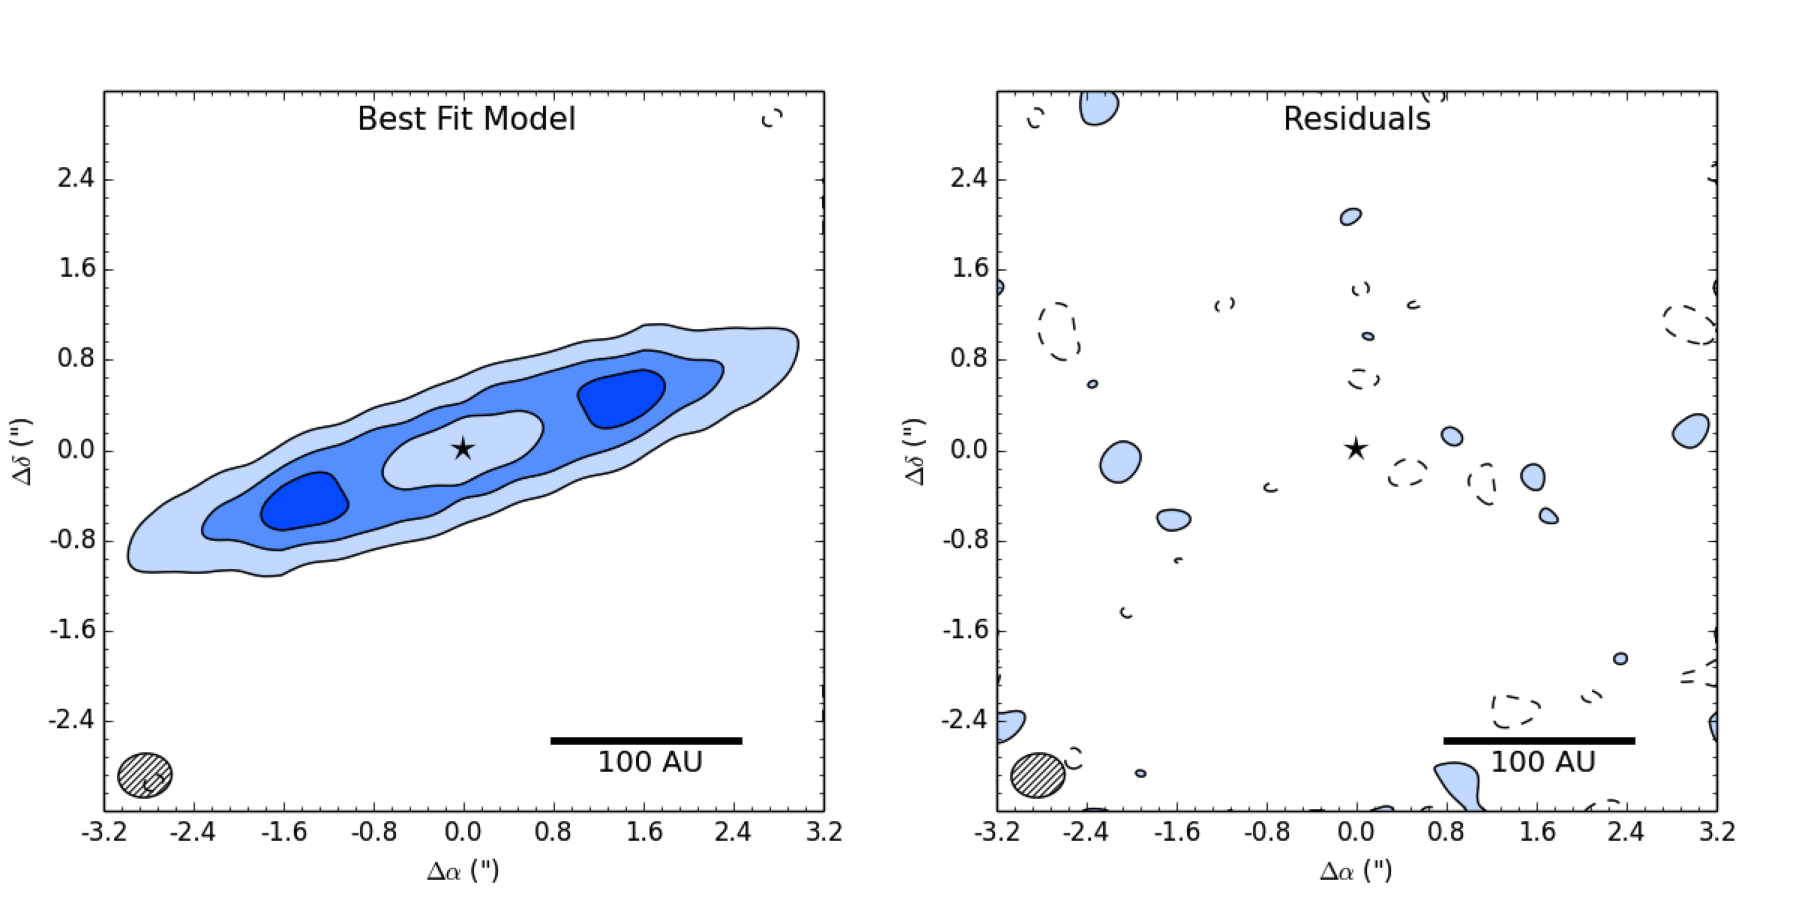
\includegraphics[width = 1\textwidth]{49CET_dPBAG_ModelResidual.png}
\caption{The model image (left) and residuals (right) for the double power law with an an additional inner disk of small grains. Contours are [-2, 2, 4, 6] $\times$ 58$\,\mu$Jy. The model leaves only a small scatter of 2$\sigma$ residuals.}
\label{fig:49CET_dPBAG_ModelResidual}
\end{figure}

\subsection{Simultaneous SED and Visibility Fit with Two Characteristic Grain Sizes}

As with the single power law model and the USDE model, we describe an inner disk of 0.1$\,\mu m$ grains extending from $R_{In}$ to $R_{Inner Disk}$ ($R_{In} + \Delta R_{Inner Disk}$) with $\Sigma_{Inner Disk} \propto r^{-1}$. We now vary $p_{1}$ from $R_{Inner Disk}$ to $R_{T}$ and vary $p_{2}$ from $R_{T}$ to $R_{Out}$, with $R_{T}$ = $R_{In} + \Delta R_{Inner Disk} + \Delta R_{T}$ and $R_{Out}$ = $R_{In} + \Delta R_{Inner Disk} + \Delta R_{T} + \Delta R_{Out}$. This model restores $p_{1}$ to the value derived from the visibility only fit within our uncertainties, and results in a model that isn't too bright at the center and doesn't leave behind positive residuals at $\sim$ 100\,AU. The best-fit model and residual images are shown in Figure \ref{fig:49CET_dPBAG_ModelResidual}, the SED is displayed in Figure \ref{fig:49CET_dPBAG_SED}, and the table of parameters is presented in Table \ref{tab:dPBAG_Table}.

\begin{figure}[t!]
\label{fig:49CET_DP_SED}
\centering
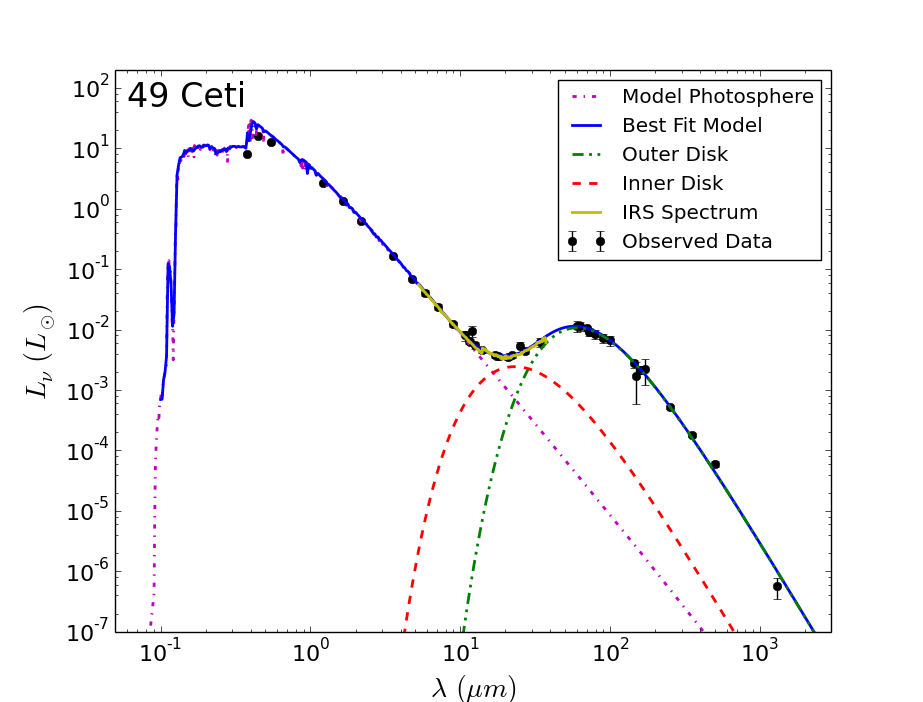
\includegraphics[width = 1\textwidth]{49CET_dPBAG_SED2.png}
\caption{The SED for the double power law model fitting the SED and visibilities for the two-part disk model. }
\label{fig:49CET_dPBAG_SED}
\end{figure}

\begin{table}[t!]
\begin{center}
    \def\arraystretch{1.37}%
    \begin{tabular}{l*{2}{c}r}
    \hline
    Parameter & Median Value $\pm$ 1$\sigma$ & Best Fit Value \\ \hline
     $R_{In}$  [AU] & 4.0$^{+1.3}_{-1.0}$ & 3.4\\  
     $\Delta R_{Inner Disk}$ [AU] & 45$^{+9}_{-11}$ & 37\\ 
     $\Delta R_{T}$ [AU] & 51$^{+12}_{-9}$ & 59\\ 
     $\Delta R_{Out}$  [AU] & 222$^{+11}_{-13}$ & 216\\ 
     log($M_{Inner Disk}$ [$M_{\oplus}$]) & -4.64$^{+0.15}_{-0.19}$ & -4.81 \\
     log($M_{Outer Disk}$ [$M_{\oplus}$]) & -1.76$^{+0.11}_{-0.11}$ &-1.72 \\
     log(a [$\mu$m]) & 0.08$^{+0.11}_{-0.12}$ & 0.10\\ 
     $\beta$ & 1.16$^{+0.06}_{-0.05}$ & 1.18\\ 
     $p_{1}$ & -1.9$^{+0.8}_{-1.4}$ & -2.0\\ 
     $p_{2}$ & 1.47$^{+0.15}_{-0.14}$ & 1.48\\ 
     $i$ [$^\circ$] & 79.3$^{+0.4}_{-0.4}$ & 79.2 \\ 
     $PA$ [$^\circ$] & -71.5$^{+0.4}_{-0.5}$ & -71.3\\
    \hline
    \end{tabular}
\end{center}
\caption{Values derived from the MCMC chain for the double-power law model with two characteristic grain sizes.}
\label{tab:dPBAG_Table}
\end{table}
%dPBAG 40x800 SED+VIS (correct sig fig) }

%%%%%

\section{Statistical Comparison of Best-fit Models}
\label{stats}

While the difference in residuals between the single power law, double power law, and USDE models for both the is not significant at any one location in the disk, these disparities may be statistically significant when considered over the whole ensemble of data and model visibilities. One method for getting a sense of whether there are any systematic errors in our models relative to the data involves deprojecting the visibilities. This radially averages them within elliptical annuli matching the disk inclination, which effectively increases the signal to noise ratio by $\sim$ 2$\pi$, although this factor also depends on the binning of our data. As can be seen in Figure \ref{fig:deprojected_DP_PL_Vis}, the best-fit visibility-only single power law model visibilities underestimate the data by a small but systematic amount between baseline lengths of $\sim$ 500 kilolambda and $\sim$ 600 kilolambda. These long baselines resolve some of the smallest angular scales, suggesting that the model might be missing some of the finer details of the disk. 

\begin{figure}
\centering
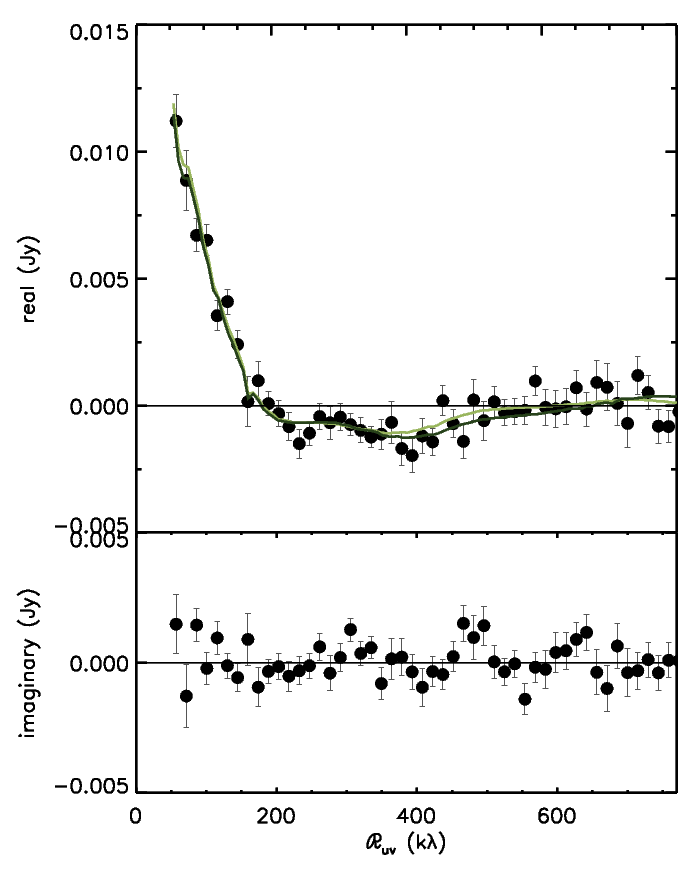
\includegraphics[width = 1\textwidth]{49CET_bestModelDeprojections_data_greenDP_blackPL.png}
\caption{The deprojected real and imaginary data visibilities are plotted in black with corresponding error bars. The green line displays the deprojected best-fit visibility-only double power law model visibilities, and the black line shows the deprojected best-fit visibility-only single power law model visibilities. A subtle but consistent systematic underestimation of the real visibilities between $\sim$ 500 kilolambda and $\sim$ 600 kilolambda is apparent for the single power law model.}
\label{fig:deprojected_DP_PL_Vis}
\end{figure}

In order to understand whether the differences between the model fits are statistically significant, we apply the Akaike Information Criterion (AIC) derived from information theory and the Bayesian Information Criterion (BIC) derived from Bayesian statistics as independent tests of whether one model is statistically better than another. A key assumption of both the AIC and BIC tests is that the posterior distribution functions are Gaussian or nearly Gaussian \citep{Lidd07}. All of our parameters from the MCMC chain are well constrained and fill out posterior distributions that fit this criteria, so we deem both tests applicable for our purposes. The AIC is defined as:

\begin{equation}
\label{eq:AIC}
\text{AIC} = -2\,\text{ln}\,\mathcal{L}_{\text{max}} + 2k
\end{equation}

where $\mathcal{L}_{\text{max}}$ is the maximum possible likelihood for the model in question (ie. the minimum $\chi^{2}$) and $k$ is the number of parameters in the model \citep{Akai74}. For $N$ data points, $\mathcal{L}_{\text{max}}$ is defined as:

\begin{equation}
\label{eq:fancyL}
\mathcal{L}_{\text{max}} = \prod_{i=1}^{N} \frac{e^{-\chi^{2}_{min}/2}}{\sqrt{2\pi} \sigma_{i}}
\end{equation} 

\begin{table}[t!]
\begin{center}
\def\arraystretch{1.37}%
\begin{tabular}{l*{3}{c}}
\hline
\hline
Model              & Single Power Law & USDE & Double Power Law  \\
\hline
$\chi^{2}_{Vis}$ & 141308.5 & 141289.617 & 141289.344   \\
%AIC            & -7.7174 & -3.7171 & -3.7171 \\
BIC           & 1689894.79 & 1689852.34 & 1689852.07 \\
%BIC           & 70.5706 & 94.1429 & 94.1429 \\ this is the top line wiki BIC val
\hline
\end{tabular}
\caption{$\chi^{2}_{Vis}$ for the single power law, USDE model, and double power law fitting just the visibilities. BIC values were calculated with Equation \ref{eq:BIC}.}
\end{center}
\label{tab:stats_table1}
\end{table}


%more easily manipulated as ln($\mathcal{L}_{\text{max}}$), which is defined as: 

%\begin{equation}
%\label{eq:fancylnL}
%\text{ln}\,\mathcal{L}_{\text{max}} =  \frac{-\chi^{2}_{min}}{2 \sqrt{2\pi}} \sum_{i=1}^{65700} \sqrt{w_{i}}
%\end{equation} 

Plugging Equation \ref{eq:fancyL} into Equation \ref{eq:AIC}, we find that the probability any differences are random between two models, $p$, is:

\begin{equation}
\label{eq:relLikelihood}
p = \text{exp}\bigg(\frac{AIC_{\text{a}}-AIC_{\text{b}}}{2}\bigg) =  \text{exp}\bigg(\frac{\chi^{2}_{min,\text{a}}-\chi^{2}_{min,\text{b}}}{2}\bigg + k_{a} - k_{b}\bigg)
\end{equation} 

%\begin{equation}
%\label{eq:relLikelihood2}
%p = \text{probability any differences are random} = \text{exp}\bigg(\frac{-\Delta \chi^{2}}{2}+\Delta \text{number of parameters}\bigg)
%\end{equation} 

%$\Delta \chi^{2}~\text{(Single Power Law With Ring vs. Double Power Law)} = 3.63 \\ p = 0.16 \approx 1\sigma$

%$\Delta \chi^{2}~\text{(Single Power Law With Ring vs. Single Power Law)} = 14.83 \\ p = 0.004 \approx 3\sigma$

%(1 $-$ prob) is the relative likelihood of model $a$ being better than model $b$. 

The BIC, first defined by \cite{Schw78_BIC}, is described as:

\begin{equation}
\label{eq:BIC}
%\text{BIC} = -2\,\text{ln}\,\mathcal{L}_{\text{max}} + k\,\text{ln}\,N
\text{BIC} = \chi^{2} + df\,\text{ln}\,N
\end{equation}

where $\chi^{2}$ is the minimum chi-squared, df is the number of degrees of freedom, and $N$ is the number of data points. If $\Delta$BIC (ie. BIC$_{a}$ - BIC_{b}$) between two models is $>$ 10, the evidence is very strong that model $b$ is better than model $a$ \citep{Kass95}. 


\begin{table}
\begin{center}
\def\arraystretch{1.37}%
\begin{tabular}{l*{3}{c}}
\hline
\hline
Model              & Single Power Law & USDE & Double Power Law  \\
\hline
 $\chi^{2}_{Vis}+$\chi^{2}_{SED}$ & 141322.080 & 141307.250 & 141310.861   \\
%AIC            & -3.7176 & 0.2826 & 0.2826 \\
BIC           & 1689884.80 & 1689846.40 & 1689850.01\\
%BIC           & 94.1424 & 117.7146 & 117.7146\\ top line wiki BIC val
\hline
\end{tabular}
\caption{$\chi^{2}_{Vis}+$\chi^{2}_{SED}$ for the single power law, USDE model, and double power law models with two characteristic grain sizes. BIC values were calculated with Equation \ref{eq:BIC}.}
\end{center}
\label{tab:stats_table2}
\end{table}

The AIC returns the same result for the USDE model and the double power law model for just the visibility fit as well as the two-part disk model, and $\Delta$BIC between these two models is less than 5 in each case, suggesting that they are statistically indistinguishable. From Equation \ref{eq:relLikelihood}, we find that the models with a surface density enhancement at $\sim$ 110\,AU are are significantly better than the single power law models at the $\sim 4\sigma$ level for the visibility-only fits and at the $\sim 3\sigma$ level for the two-part disk models. Complementing this result, $\Delta$BIC $\sim$ 40 for comparing both the USDE and double power law to the single power law, so with a high degree of confidence, we posit that the models of the surface density with peak values at r $\sim$ 110\,AU best represent the physical nature of 49 Ceti's dust disk. 

%For the visibility-only fits, Equation \ref{eq:relLikelihood} shows that the both the USDE and double power law models are better than the single power law model at the $\sim$ 4$\sigma$ level (will calculate exact value later), and that there is no statistical difference between USDE and double power law models.  

%are truer to the physical 
%0.135 times as likely as the single power law to ``minimize the information loss" for both the visibility-only and two-part best-fit models.  $<<$ what does this really mean tho??? 

From a philosophical standpoint, further evidence for the significance of the density enhancement at $\sim$ 110\,AU comes from the fact that both of our more complex models could have effectively ignored the additional parameters---the USDE model could have prescribed $M_{Ring}$ = 0 and had its values for the power law and transition radius match those of the best-fit single power law model, and the double power law model could have settled on two decreasing power laws such that the surface density for the outer disk would match that of the single power law---but they didn't. Rather, within our derived uncertainties, they ascribe the peak of the surface density to be at the same radius (Figure \ref{fig:densityDistr}). Even though it seems in this plot that the turnover from inner disk to outer disk for the single power law is close to the radius of the peak density, it settles on $R_{Inner Disk}$ = 73 $\pm$ 3\,AU, significantly smaller than the peak surface density at a radius of 114$^{+3}_{-3}$\,AU and 100$^{+15}_{-14}$\,AU for the USDE and double power law models, respectively. 

%$\sim$ 110AU in the double power and USDE models. 

\begin{figure}
\centering
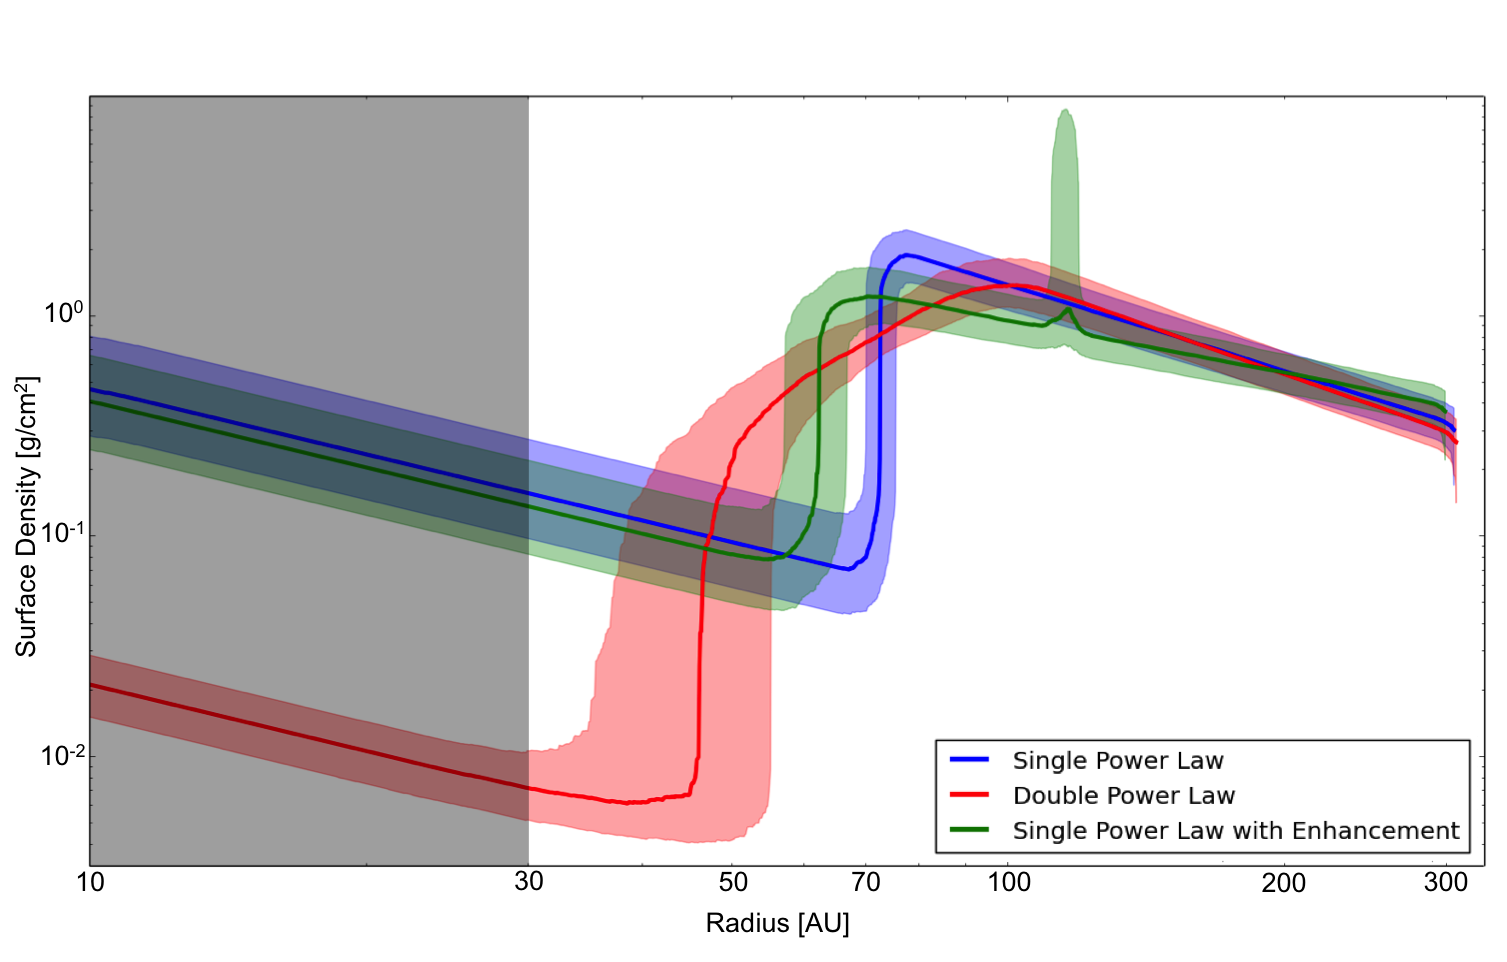
\includegraphics[width = 1\textwidth]{49CET_SDD2_withShaded_oldPerson.png}
\caption{The best-fit surface density distributions for the single power law, USDE, and double power law models with two characteristic grain sizes are shown as thick lines, with their uncertainties ($\pm$ 1$\sigma$) displayed as the respective shaded color. The grey shaded region denotes the spatial resolution of our ALMA data, helping to exhibit that the surface density distribution is not well characterized for the inner disk, where $\Sigma_{\text{Inner Disk}} \propto r^{-1}$ by definition and the scaling is only affected by the fit to the SED.}
\label{fig:densityDistr}
\end{figure}

%See Tables \ref{tab:49CET_nOBAG_Table}, \ref{tab:bBBAG_Table}, and \ref{tab:dPBAG_Table} for exact values related to the plotted parameters.


%e^-chi2/2 / root2pi(product of square root of weights)

%flux is spread around imaging
%radial averaging improves SNR by 2pi
%see that plot systematics
%at small scales

%clean does weird things to noise in images
%noise in vis isn't equal to noise in iamge
%don't understand how noise transfers through clean process



%%%%%%

%Transition radius = transition radius
%outer radius = inner radius + delta rOut



%%%%


\section{Mid-Infrared Properties}
\label{MidIR}

\begin{figure}[t!]
\centering
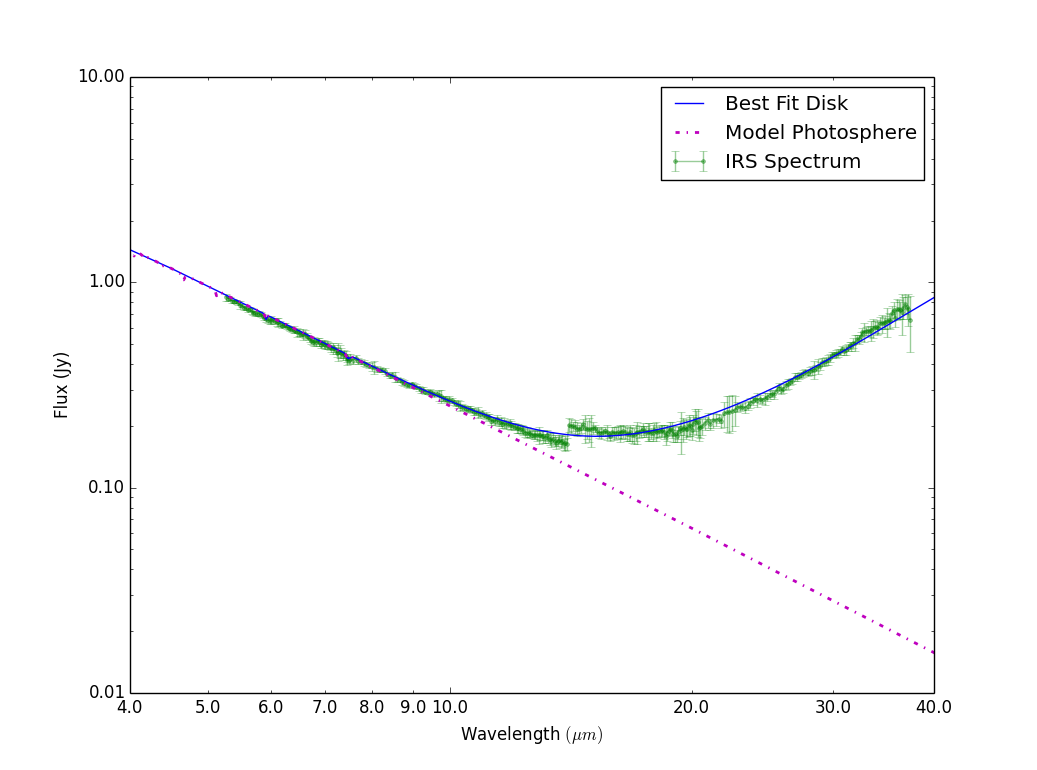
\includegraphics[width = 1\textwidth]{49CET_IRS_Window.png}
\caption{The IRS spectrum of 49 Ceti is plotted in green along with each point's statistical uncertainty. The absolute calibration uncertainty used in fitting the SED, assumed to be 10$\%$ of the flux measurement, is not displayed. A sample best-fit disk and the model photosphere are plotted for reference.}
\label{fig:49CET_IRS_Window}
\end{figure}


The detail and accuracy of the 360 points that make up the $\it{Spitzer}$ IRS spectrum, presented in Figure \ref{fig:49CET_IRS_Window}, allow us to see characteristic emission features of silicate grains (or the lack thereof). The jump at 14$\,\mu m$ in the spectrum is not an emission feature, but rather a calibration issue resulting from the fact there are two separate sub-modules being used to take spectra within IRS (one from 5 - 14$\,\mu m$, the other from 14 - 40$\,\mu m$). We do not see any emission features at 10$\,\mu m$, where emission due to silicate grains usually peaks, but the implications of this absence of silicate emission is so far unclear due to insufficient observational constraints. 

Silicate features are most apparent when the emitting grains are smaller than $\sim$ 1$\,\mu m$ \citep{Papo83}, but  \cite{Natt07} show that 10$\,\mu m$ spectral features are also apparent in the emission of 200-600K grains smaller than a few microns. Our best fit models suggest an inner radius of $\sim$ 5\,AU, which is right on the border of where we expect to find grains at this temperature,  so it might be that there simply aren't grains with the right properties to display any mid-IR features. 

% but can be washed out if they are not the dominant emitters. 
%In addition, even if there are grains of this size, if the crystal lattice structure is uneven, the emission feature will be less pronounced. \cite{Natt07} suggest that the 10$\,\mu m$ spectral region probes 200-600K grains smaller than a few microns confined to the disk surface within $\sim$ 10AU of the star for protoplanetary disks and within $\sim$ 1AU from the star in the case of T Tauri stars. Our best fit model suggests an inner radius of ?????, which is right on the border of where we expect to find these grains with these characteristics, so it might be that there simply aren't grains with the right properties to display any mid-IR features. 

It is possible that the percentage of silicate grains is low in 49 Ceti's disk, and that the composition of the grains is dominated by carbon. The high albedo of silicate grains is usually responsible for reflecting enough light to be seen in scattered light imaging, but the non-detection of the disk at separations $>$ 1.6 arcsec \citep{Wein99} in scattered light provides evidence that silicates may not dominate the composition. In addition, \cite{Robe14} find an extreme carbon overabundance relative to iron, suggesting that the disk is volatile-rich. However, $\beta$ Pic shows the same overabundance of carbon, but it is easily seen in scattered light with \textit{HST}. 

%Because silicates tend to have much higher albedos than carbon-based grains, the non-detection of any scattered light at separations $>$1.6$''$ \ref{Wein99} suggests that 
%All of these are possibilities for 49 Ceti's disk, but it is unclear what the dominant reason is that we do not observe any silicate features. 


